\graphicspath{{chapters/gradient_descent/}}


\chapter{Scaling CCA: Stochastic Methods for High-Dimensional Subspace Learning}\label{ch:gradient_descent}
\epigraph{It seems easier to train a bi-directional LSTM with attention than to compute the SVD of a large matrix}{Chris Ré}\citep{gemp2021}
\minitoc
% chktex-file 44
% chktex-file 3
\section*{Preface}
The content of this chapter is based on a series of papers~\citep{chapman2022generalized, chapman2023efficient} as well as a NeurIPS workshop paper~\citep{chapman2023cca}.
I am grateful to my co-authors Lennie Wells and Ana Lawry Aguila for their contributions to this work.
I conceived the original idea of developing new stochastic algorithms based on the GEP formulation CCA using the GEP formulation, and developed a number of methods that appeared to perform well empirically including writing all of the code and preliminary proofs. 
Lennie formalised the Eckart-Young-Mirsky theorem-based objective and developed the theoretical results, while Ana provided the processed data from the UK Biobank and ran the UK Biobank experiments.
In the interests of communicating my contribution, in this chapter I include the results from the papers but refer the reader to the original papers for Lennie's detailed derivations and proofs.

\section{Introduction}
Generalized Eigenvalue Problems (GEPs) are fundamental to a wide range of machine learning algorithms, including Canonical Correlation Analysis (CCA), Partial Least Squares (PLS), Principal Component Analysis (PCA), Independent Component Analysis (ICA), and Linear Discriminant Analysis (LDA). Solving high-dimensional GEPs is a critical challenge in many applications, as classical algorithms often struggle with the computational complexity and numerical instability that arise when dealing with large-scale datasets. This has motivated the development of stochastic algorithms that aim to approximate the solutions of GEPs in a more efficient and scalable manner.
Stochastic algorithms for simple Eigenvalue Problems (EPs), where the matrix $B$ in the GEP is the identity matrix, have been extensively studied and have shown promising results \citep{arora2012stochastic,arora2016stochastic}. These algorithms not only offer computational advantages but also introduce a form of implicit regularization through the noise in the stochastic updates, which can be particularly beneficial in high-dimensional settings. The regularizing effect of stochastic algorithms has been shown to improve generalization performance and robustness to noise, making them an attractive alternative to batch learning algorithms.
However, when it comes to solving more complex GEPs, such as those arising in CCA and PLS, the existing stochastic algorithms have some limitations that hinder their practical applicability. For instance, the $\gamma$-EigenGame algorithm \citep{gemp20,gemp2021} requires the tuning of a hyperparameter $\gamma$ that controls the trade-off between computational efficiency and the accuracy of the stochastic updates. Finding the optimal value of this hyperparameter can be challenging and may vary depending on the problem and the data, making the algorithm less convenient to use in practice.
Another limitation is that some stochastic algorithms, like the Stochastic Generalized Hebbian Algorithm (SGHA) \citep{chen2019constrained}, rely on heuristic primal-dual update rules rather than a principled optimization framework. This makes it difficult to integrate these algorithms with more sophisticated optimizers like Adam \citep{kingma2014adam}, which have been shown to improve convergence speed and stability in many machine learning applications.
To address these limitations and provide a more principled and robust approach to solving GEPs in the stochastic setting, we propose a novel formulation of the CCA problem based on the Eckhart--Young--Minsky inequality \citep{stewart_matrix_1990}. Our formulation leads to a new objective function that characterizes the top-$K$ subspace of GEPs, including CCA as a special case. Importantly, this objective function is unconstrained and can be optimized using standard stochastic gradient descent or batch gradient descent methods, making it compatible with modern optimization techniques.
The key advantages of our proposed approach are:
\begin{itemize}
    \item It provides a unified framework for solving a wide range of GEPs using a single unconstrained objective function, making it applicable to CCA, PLS, PCA, ICA, LDA, and other problems that can be formulated as GEPs.
    \item The objective function can be efficiently optimized using stochastic gradient descent or batch gradient descent, allowing for seamless integration with state-of-the-art optimizers like Adam.
    \item The stochastic nature of the optimization introduces implicit regularization, which can improve the generalization performance and robustness of the learned subspaces.
    \item The approach is more principled and theoretically grounded compared to heuristic primal-dual update rules used in some existing stochastic algorithms.
\end{itemize}

The rest of this chapter is organized as follows: Section \ref{sec:background-unified} provides background on GEPs and existing methods for solving them. Section \ref{sec:contributions} introduces our novel Eckhart-Young inspired objective and the GEP-EY algorithm. Section \ref{sec:experiments} presents experimental results on various datasets. Finally, Section \ref{sec:discussion} discusses limitations, future work, and concludes the chapter.

\section{Background: Efficient Solutions to GEPs}\label{sec:background-unified}
\subsection{Solving High-Dimensional Generalized Eigenvalue Problems}
Generalized Eigenvalue Problems (GEPs) play a crucial role in many machine learning algorithms, including Canonical Correlation Analysis (CCA), Partial Least Squares (PLS), Principal Component Analysis (PCA), Independent Component Analysis (ICA), and Linear Discriminant Analysis (LDA). A GEP is defined by two matrices $A$ and $B$, where the goal is to find a vector $u$ and a scalar $\lambda$ that satisfy the equation:
\begin{equation}
Au = \lambda Bu
\end{equation}
The vector $u$ is called the generalized eigenvector, and the scalar $\lambda$ is called the generalized eigenvalue. In the special case where $B$ is the identity matrix, the GEP reduces to a standard Eigenvalue Problem (EP).
Solving GEPs becomes challenging when dealing with high-dimensional data, where the matrices $A$ and $B$ can be very large. The computational complexity of classical algorithms for solving GEPs, such as the power method, scales cubically with the size of the matrices, making them infeasible for large-scale problems. Moreover, when the matrices are ill-conditioned or nearly singular, these algorithms can suffer from numerical instability, leading to inaccurate or unreliable solutions.

\subsection{Unified GEP formulation for CCA, Ridge CCA, PLS, and PCA}
As discussed in \ref{ch:background}\ref{sec:classical-subspace-learning-algorithms}, CCA, ridge-regularized CCA, PLS, and even PCA can be formulated as GEPs with specific structures. This unified formulation involves block matrices $A$ and $B_\alpha$ defined as:
\begin{align}
A^{(ij)} &= \Cov(X\sps{i}, X\sps{j}) \text{ for } i \neq j, \
B_\alpha^{(ii)} &= \alpha_i I_{D\sps{i}} + (1-\alpha_i) \Var(X\sps{i}),
\end{align}
where $\alpha \in [0,1]^I$ is a vector of ridge penalty parameters, $X\sps{i}$ represents the $i$-th view of the data, and $D\sps{i}$ is the dimensionality of the $i$-th view.
By adjusting the values of $\alpha$, we can recover various subspace learning methods:

Pure CCA: Setting $\alpha_i = 0 : \forall i$ recovers the classic CCA problem.
Ridge Extensions: Smoothly transitioning to ridge-regularized CCA or PLS by selectively adjusting values within $\alpha$.
PCA Subsumption: PCA emerges as a single-view form of ridge-regularized PLS.

This unified formulation allows us to focus on solving the core CCA problem, with the understanding that the insights and solutions developed will naturally generalize to the entire family of methods and GEPs more generally.

\subsection{Classical Methods for Solving CCA}
\subsubsection{Eigendecomposition-based Solution}
One common technique to solve the GEP for CCA is to transform it into a standard eigenvalue problem:
\begin{equation}
B^{-\frac{1}{2}} A B^{-\frac{1}{2}} y = \lambda y
\end{equation}
followed by eigendecomposition. This approach is based on the observation that if $(u, \lambda)$ is a generalized eigenpair of $(A, B)$, then $(B^{-\frac{1}{2}}u, \lambda)$ is an eigenpair of $B^{-\frac{1}{2}} A B^{-\frac{1}{2}}$.
An alternative approach is to solve the eigenvalue problem:
\begin{equation}
B^{-1} A v = \lambda v
\end{equation}
However, this approach requires computing the inverse of $B$, which can be numerically unstable and computationally expensive, especially when $B$ is ill-conditioned or nearly singular. In contrast, the $B^{-\frac{1}{2}} A B^{-\frac{1}{2}}$ formulation only requires computing the square root of $B$, which can be done more efficiently and stably using techniques like the Cholesky decomposition.
Nonetheless, both approaches have a computational complexity of $\mathcal{O}((d_1+d_2)^3)$ and may suffer from numerical instability, especially when $B$ is ill-conditioned or nearly singular.

\subsubsection{Classical Iterative Algorithms}
Classical iterative algorithms, such as the power method, Sanger's rule (Generalized Hebbian Algorithm), and Oja's rule, can be used to solve the GEP for CCA. These algorithms are based on the idea of iteratively updating the eigenvector estimates using matrix-vector multiplications.
The power method is a simple iterative algorithm for finding the dominant eigenvector of a matrix $A$. The update rule for the power method is:
\begin{align}
u \leftarrow \frac{A u}{|A u|}
\end{align}
where $u$ is the current estimate of the dominant eigenvector. The power method converges to the dominant eigenvector of $A$ under mild conditions.
Sanger's rule, also known as the Generalized Hebbian Algorithm (GHA), is an iterative learning rule for finding the principal components of a data set. It can be written as:
\begin{align}
U \leftarrow U + \eta \left( A U - U \text{tril}(U^T A U) \right)
\end{align}
where $\text{tril}(\cdot)$ denotes the lower triangular part of a matrix.
Oja's rule, a simplified version of Sanger's rule, can be written as:
\begin{align}
U \leftarrow U + \eta \left( A U - U (U^T A U) \right)
\end{align}
To maintain orthogonality of the eigenvectors during the iterative updates, Oja's rule can be combined with a QR decomposition step:
\begin{align}
U \leftarrow U + \eta \left( A U - U (U^T A U) \right) \
U \leftarrow \text{qr}(U)
\end{align}
where $\text{qr}(\cdot)$ denotes the QR decomposition, which factorizes a matrix into an orthogonal matrix $Q$ and an upper triangular matrix $R$. By using only the orthogonal matrix $Q$, we ensure that the eigenvectors remain orthogonal throughout the iterative process. Alternatively, other orthogonalization techniques such as the Gram-Schmidt process can be employed.
These iterative algorithms can be extended to solve the generalized eigenvalue problem $A U = B U \Lambda$, where $B$ is a positive definite matrix. The update rule for this problem is:
\begin{align}
U \leftarrow U + \eta \left( A U - B U \text{tril}(U^T A U) \right)
\end{align}
which subsumes the original GHA as a special case when $B=I$.
While these classical iterative algorithms can be computationally efficient, especially for sparse or structured matrices, they may suffer from slow convergence and sensitivity to initialization.

\subsubsection{PCA-CCA}
To reduce the computational complexity of solving the GEP for CCA, the PCA-CCA method first applies PCA to each view of the data separately and then solves the GEP in the reduced space. This approach has two main steps:

\begin{itemize}
    \item Apply PCA to each view: Compute the top $K_1$ and $K_2$ principal components for each view, with complexity $\mathcal{O}(d_1^3 + d_2^3)$.
    \item Solve the GEP in the reduced space: Solve the GEP in the reduced space of size $(K_1 + K_2) \times (K_1 + K_2)$, with complexity $\mathcal{O}((K_1 + K_2)^3)$.
\end{itemize}

The overall complexity of PCA-CCA is thus $\mathcal{O}(d_1^3 + d_2^3 + (K_1 + K_2)^3)$, which can be significantly lower than the direct solution when $K_1 \ll d_1$ and $K_2 \ll d_2$.
However, it's important to note that even the PCA step can be computationally expensive for high-dimensional data. In the case where the number of samples $n$ is smaller than the dimensionalities $d_1$ and $d_2$, the maximum number of principal components is $K_1 = K_2 = n$. The complexity of PCA in this case is $\mathcal{O}(n^3 + n^3)$, and the overall complexity of PCA-CCA becomes $\mathcal{O}(2n^3 + (2n)^3) = \mathcal{O}(10n^3)$. While this is lower than the direct solution, it can still be prohibitive for large sample sizes.
\subsubsection{Kernel CCA}
Kernel CCA (KCCA) is another approach that offers computational advantages for high-dimensional data. KCCA maps the original data to a high-dimensional feature space using a kernel function and then performs CCA in that space. The main advantage of KCCA is that its complexity scales with the number of samples $n$ rather than the dimensionalities $d_1$ and $d_2$.
The optimization problem for KCCA can be written as:
\begin{align}
& \alpha_{\text{opt}} = \underset{\alpha}{\mathrm{argmax}} { \alpha\sps{1} K\spsT{1} K\sps{2} \alpha\sps{2} } \
& \text{subject to:} \notag \
& \alpha\sps{1} K\spsT{1} K\sps{1} \alpha\sps{1} = 1 \notag \\
& \alpha\sps{2} K\spsT{2} K\sps{2} \alpha\sps{2} = 1 \notag
\end{align}
where $\alpha\sps{i}$ are dual variables, $K\sps{i}$ are kernel matrices defined as $K\sps{i} = \phi(X\sps{i})\phi(X\sps{i})^T$, and $\phi(\cdot)$ is a nonlinear mapping function.
The complexity of KCCA is $\mathcal{O}(n^3)$, which can be much lower than the direct solution when $d_i > n$. However, KCCA has some significant drawbacks:
\begin{itemize}
    \item The need to store and manipulate the kernel matrices, which have size $n \times n$. This can be memory-intensive for large sample sizes.
    \item The requirement to access all training data at test time, which raises concerns about efficiency and scalability.
    \item The difficulty in interpreting the results in the original feature space, as the learned projections are in the high-dimensional kernel space.
\end{itemize}

In summary, classical methods for solving CCA offer various trade-offs between computational complexity, numerical stability, and interpretability. However, these methods may still be prohibitively expensive for high-dimensional data, motivating the development of stochastic algorithms that can efficiently approximate the solution of the CCA problem.

\subsection{Stochastic Algorithms for CCA}

The principle of empirical risk minimization (ERM) forms the basis for many learning algorithms. ERM involves evaluating and optimizing the performance of an algorithm over a known, fixed dataset. This approach is grounded in the law of large numbers: while we cannot know the true risk associated with the underlying data distribution, we can estimate and optimize the algorithm's performance on a known set of training data, referred to as the empirical risk \citep{vapnik1999nature}.

Traditionally, ERM algorithms process the entire dataset in a batch, updating the model parameters based on the full dataset. Stochastic algorithms extend the ERM framework to handle large-scale datasets by processing the data in small batches or even one sample at a time. 

Stochastic methods offer several advantages. They allow us to handle large-scale datasets that may not fit in memory, provide implicit regularization through the noise in the stochastic updates, and often lead to better generalization by approximating the population objective rather than overfitting to the empirical risk.

While stochastic optimization has proven highly effective for solving unconstrained objectives in machine learning, its application to Generalized Eigenvalue Problems (GEPs) and Canonical Correlation Analysis (CCA) presents unique challenges. The primary difficulty lies in handling the data-dependent constraint $U^\top B U = I$, which is essential for ensuring the orthogonality of the learned subspaces. This constraint is particularly challenging to address in the stochastic setting, as $B$ is not directly accessible and must be estimated from random samples, introducing additional uncertainty into the optimization process.

\subsubsection{Stochastic Power Method for PLS}
\citet{arora2016stochastic} demonstrate that PLS can be approximated by applying a stochastic power method. The stochastic power method is a simple iterative algorithm that updates the estimates of the left and right singular vectors $U^{(1)}$ and $U^{(2)}$ using the following rules:
\begin{align*}
U^{(1)}_t &= \mathcal{P}_{\text{orth}} \left( U^{(1)}_{t-1} + \eta_t X_t^{(1)} (X_t^{(2)})^\top U^{(2)}_{t-1} \right), \\
U^{(2)}_t &= \mathcal{P}_{\text{orth}} \left( U^{(2)}_{t-1} + \eta_t X_t^{(2)} (X_t^{(1)})^\top U^{(1)}_{t-1} \right),
\end{align*}
where $\mathcal{P}_{\text{orth}}(\cdot)$ represents an orthogonal projection operator that projects a vector or matrix onto the space orthogonal to the current subspace, $X_t^{(1)}$ and $X_t^{(2)}$ are the new data points at time $t$, and $\eta_t$ is the learning rate.
Intuitively, the update rule for $U^{(1)}_t$ can be understood as follows:

The term $X_t^{(1)} (X_t^{(2)})^\top U^{(2)}_{t-1}$ computes the correlation between the new data point $X_t^{(1)}$ and the current estimate of the right singular vector $U^{(2)}_{t-1}$, weighted by the corresponding $X_t^{(2)}$.
This correlation term is then added to the current estimate of the left singular vector $U^{(1)}_{t-1}$, effectively updating it in the direction that maximizes the covariance between the views.
The orthogonal projection operator $\mathcal{P}_{\text{orth}}(\cdot)$ ensures that the updated estimate remains orthogonal to the previous estimates, preventing the algorithm from converging to a suboptimal solution.

The update rule for $U^{(2)}_t$ follows a similar logic, with the roles of $X_t^{(1)}$ and $X_t^{(2)}$ reversed.

The stochastic power method has a low computational complexity of $\mathcal{O}(k(d_1+ d_2))$ per iteration, where $k$ is the number of components being estimated. However, it has some limitations:

Convergence is not guaranteed, as the algorithm may oscillate or diverge in some cases.
The orthogonal projection step does not extend naturally to the CCA problem, where the constraints involve the matrix $B$ (i.e., $U^\top B U = I$) rather than the identity matrix (i.e., $U^\top U = I$).

Despite these limitations, the stochastic power method provides valuable insights into the design of stochastic algorithms for CCA and serves as a foundation for more advanced methods.
\subsubsection{Stochastic Generalized Hebbian Algorithm (SGHA)}
The Stochastic Generalized Hebbian Algorithm (SGHA), proposed by \citet{chen2019constrained}, is an extension of the Generalized Hebbian Algorithm (GHA) to the stochastic setting. SGHA aims to find the top-$k$ generalized eigenvectors of a matrix pair $(A, B)$, where $A$ is symmetric and $B$ is symmetric positive definite.
SGHA formulates the constrained optimization problem for the top-$k$ subspace as:
\begin{align}
\min_{U} -\Tr \left(U^T A U\right) \quad \text{subject to} \quad U^T B U = I
\end{align}
Using Lagrange multipliers, this constrained problem can be transformed into an unconstrained one:
\begin{align}
\min_{U} -\Tr\left(U^T A U \right) + \lambda \left(U^T B U - I\right)
\end{align}
Differentiating with respect to $U$ and $\lambda$ and setting the derivatives to zero yields the stationary points:
\begin{align}
2 A U - 2 B U \lambda = 0 \quad \text{and} \quad U^T B U - I = 0 \
\implies \lambda = U^T A U
\end{align}
Based on these stationary points, SGHA proposes a primal-dual update rule:
\begin{align}
U \leftarrow U - \eta \left( A U - B U \lambda \right) \
\lambda \leftarrow \left( U^T A U \right)
\end{align}
where $\eta$ is a learning rate.
These updates can be combined into a single update rule:
\begin{align}
U \leftarrow U - \eta \left( A U - B U \left( U^T A U \right) \right)
\end{align}
Intuitively, the SGHA update rule can be understood as follows:

The term $A U$ computes the correlation between the current estimate of the generalized eigenvectors $U$ and the data matrix $A$.
The term $B U \left( U^T A U \right)$ serves as a correction term that ensures the orthogonality of the eigenvectors with respect to the matrix $B$. The matrix $\left( U^T A U \right)$ can be interpreted as an estimate of the generalized eigenvalues.
The difference between these two terms is then used to update the current estimate of the eigenvectors $U$ in the direction that maximizes the objective function.

SGHA has a computational complexity of $\mathcal{O}(k^2(d_1+ d_2))$ per iteration, which is higher than that of the stochastic power method but still much lower than the batch methods.
While SGHA is simple to implement, it relies on a heuristic primal-dual update rule rather than a principled optimization framework. This makes it difficult to integrate with more sophisticated optimizers like Adam \citep{kingma2014adam}, which have been shown to improve convergence speed and stability in many machine learning applications.
\subsubsection{$\gamma$-EigenGame for CCA}
The $\gamma$-EigenGame, proposed by \citet{gemp20,gemp2021}, is a stochastic algorithm for CCA inspired by the EigenGame algorithm for PCA. The key idea behind the $\gamma$-EigenGame is to view the generalized eigenvectors as competing players in a game, where each player tries to maximize its own utility function.
In this game-theoretic formulation, the utility function of each player (eigenvector) $u_i$ consists of a reward term and a penalty term:
\begin{align}
\max_{u_i} \overbrace{\frac{u_i^TAu_i}{u_i^TBu_i}}^{\text{reward}} - \overbrace{\sum_{j < i} \frac{(u_j^TAu_j)(u_i^TBu_j)^2}{(u_j^TBu_j)^2(u_i^TBu_i)}}^{\text{penalty}}
\end{align}
The reward term $\frac{u_i^TAu_i}{u_i^TBu_i}$ encourages the eigenvector $u_i$ to align with the direction of maximum correlation between the views, while the penalty term $\sum_{j < i} \frac{(u_j^TAu_j)(u_i^TBu_j)^2}{(u_j^TBu_j)^2(u_i^TBu_i)}$ discourages $u_i$ from aligning with the directions already captured by the previous eigenvectors $u_j$ for $j < i$.
The $\gamma$-EigenGame proposes an update rule for each eigenvector $u_i$ based on this utility function. In the stochastic setting, the algorithm introduces an additional hyperparameter $\gamma$ that controls the trade-off between computational efficiency and the accuracy of the stochastic updates. The update rule is modified to use a rolling average of the matrix $B$, which helps to reduce the computational complexity and memory requirements of the algorithm.
While the $\gamma$-EigenGame has shown promising results in practice, it still requires the tuning of both the hyperparameter $\gamma$ and a learning rate, which can be challenging and may depend on the specific problem and data at hand.
Moreover, the use of a rolling average of the matrix $B$ introduces additional approximation error and may not fully capture the uncertainty in the stochastic orthogonality constraint $U^\top B U = I$.

\subsubsection{Benefits and Limitations of Stochastic Algorithms}
Stochastic algorithms offer several benefits over batch methods for solving CCA problems, such as computational efficiency, implicit regularization, and online learning capabilities. However, they also have some limitations, particularly in the context of stochastic GEPs and stochastic CCA:

Convergence: The convergence of stochastic algorithms can be slower than batch methods, especially in the presence of noise or when the data is highly correlated. The choice of learning rate and mini-batch size can have a significant impact on the convergence speed and stability.
Hyperparameter tuning: Most stochastic algorithms require the tuning of several hyperparameters, such as the learning rate, mini-batch size, and regularization parameters. The optimal values of these hyperparameters can vary depending on the problem and the data, making it challenging to achieve consistent performance across different datasets.
Stochastic orthogonality constraint: The data-dependent constraint $U^\top B U = I$ becomes stochastic when $B$ is replaced by a sample estimate, introducing additional uncertainty and approximation error. Existing stochastic algorithms may not fully account for this uncertainty, leading to suboptimal solutions or slower convergence.
Theoretical guarantees: The theoretical guarantees for stochastic algorithms are often weaker than those for batch methods, particularly in terms of the rate of convergence and the quality of the solution. The analysis of their convergence properties can be complex and may depend on strong assumptions about the data distribution and the noise.

Despite these limitations, stochastic algorithms have shown promising results in practice and have become increasingly popular for solving large-scale CCA problems. The development of more principled and theoretically grounded stochastic algorithms that can handle the stochastic orthogonality constraint remains an active area of research.
In the next section, we will introduce a novel stochastic algorithm for CCA based on the Eckart-Young-Mirsky theorem, which aims to address some of the limitations of existing methods and provide a more principled and robust approach to solving high-dimensional CCA problems in the presence of stochastic constraints.

\section{Methods: GEP-EY, An Efficient Algorithm for Generalized Eigenvalue Problems}\label{sec:contributions}
This section introduces GEP-EY, a novel algorithm for solving Generalized Eigenvalue Problems (GEPs), with a particular focus on Canonical Correlation Analysis (CCA) and Partial Least Squares (PLS). The algorithm stems from a new perspective on GEPs: optimizing an Eckart-Young inspired objective that characterizes the GEP solution.

\subsection{A New Perspective: Eckhart-Young Inspired Objective for GEPs}

\subsubsection{Formulation and Intuition}
At the core of our approach is the reformulation of GEPs as an unconstrained optimization problem. This reformulation is inspired by the Eckhart-Young-Mirsky theorem, which is fundamental in matrix approximation theory.

The Eckhart-Young-Mirsky theorem states that the best rank-$K$ approximation of a matrix \(M\) in the Frobenius norm is given by its truncated singular value decomposition (SVD). Specifically, if \(M = U \Sigma V^\top\) is the SVD of \(M\), then the optimal rank-$K$ approximation is \(M_K = U_K \Sigma_K V_K^\top\), where \(U_K\), \(\Sigma_K\), and \(V_K\) are the matrices containing the top $K$ singular vectors and singular values.

We apply a similar approach to the generalized eigenvalue problem (GEP) defined by matrices \(A\) and \(B\). By considering the eigen-decomposition of \(B^{-\frac{1}{2}} A B^{-\frac{1}{2}}\), we can derive a new objective function for characterizing the top-$K$ subspace of the GEP.

\begin{restatable}[Eckhart-Young inspired objective for GEPs]{proposition}{EYcharac}
    \label{prop:EY-charac}
    The top-$K$ subspace of the GEP $(A,B)$ can be characterized by minimizing:
    \begin{align}\label{eq:EY-charac}
    \LEYGEP(U) \defeq \tr \left( - 2U^\top A U + \left(U^\top B U\right) \left(U^\top B U\right) \right)
    \end{align}
    over $U \in \R^{D \times K}$, with a minimum value of $- \sum_{k=1}^K \lambda_k^2$, where $(\lambda_k)$ are the generalized eigenvalues.
\end{restatable}
    
This objective intuitively balances maximizing between-view correlations and minimizing within-view variances.

\paragraph{Sketch of the Proof:}
To provide some intuition, we sketch the key steps in the proof, with full details available in our supplementary material.

\begin{enumerate}
    \item \textbf{Matrix Approximation and SVD:} Begin with the Eckhart-Young-Mirsky theorem, which gives the best rank-$K$ approximation in the Frobenius norm for any matrix using its SVD. The theorem states that for a matrix \(M \in \R^{d \times d}\), the best rank-$K$ approximation \(M_K\) is obtained by truncating the SVD of \(M\).
    
    \item \textbf{Transformation of GEP:} For the GEP defined by matrices \(A\) and \(B\), consider the transformation \(M = B^{-\frac{1}{2}} A B^{-\frac{1}{2}}\). The eigenvalues and eigenvectors of \(M\) are related to the generalized eigenvalues and eigenvectors of \((A,B)\). This transformation simplifies the problem, as \(M\) is symmetric.

    \item \textbf{Objective Reformulation:} By focusing on the top-$K$ eigenvalues and eigenvectors, we can reformulate the problem as an unconstrained optimization problem. Specifically, consider the objective function:
    \[
    \| M - \tilde{W} \tilde{W}^T \|_F^2.
    \]
    Since \(M\) is symmetric, the optimal \(\tilde{W}\) is of the form \(W = W_K \Lambda_K^{\frac{1}{2}} O_K\), where \(W_K\) contains the top-$K$ eigenvectors, \(\Lambda_K\) contains the corresponding eigenvalues on the diagonal, and \(O_K\) is an orthogonal matrix.

    \item \textbf{Transformation under reparameterisation:} Consider how this expression transforms under the reparameterisation \(\tilde{W} = B^{\frac{1}{2}} \tilde{U}\). We get:
    \[
    \| M - \tilde{Z} \tilde{Z}^T \|_F^2 = \| B^{-\frac{1}{2}} A B^{-\frac{1}{2}} - B^{\frac{1}{2}} \tilde{U} \tilde{U}^T B^{\frac{1}{2}} \|_F^2.
    \]

    \item \textbf{Simplifying the Objective:} Simplifying the expression, we use the properties of the Frobenius norm and the cyclic property of the trace:
    \begin{align*}
        \| B^{-\frac{1}{2}} A B^{-\frac{1}{2}} - B^{\frac{1}{2}} \tilde{U} \tilde{U}^T B^{\frac{1}{2}} \|_F^2 &= \| B^{-\frac{1}{2}} A B^{-\frac{1}{2}} \|_F^2 - 2 \tr(B^{-\frac{1}{2}} A B^{-\frac{1}{2}} B^{\frac{1}{2}} \tilde{U} \tilde{U}^T B^{\frac{1}{2}}) \\
        &\quad + \tr((B^{\frac{1}{2}} \tilde{U} \tilde{U}^T B^{\frac{1}{2}})^2) \\
        &= \| B^{-\frac{1}{2}} A B^{-\frac{1}{2}} \|_F^2 - 2 \tr(\tilde{U}^T A \tilde{U}) + \tr((\tilde{U}^T B \tilde{U})^2).
    \end{align*}

    \item \textbf{Final Reformulation:} This leads to the final form of the objective function:
    \[
    \LEYGEP(U) \defeq \tr \left( - 2U^\top A U + \left(U^\top B U\right) \left(U^\top B U\right) \right),
    \]
    where \(U = \tilde{W}\).

    This objective intuitively balances maximizing between-view correlations (captured by \(U^\top A U\)) and minimizing within-view variances (captured by \((U^\top B U)(U^\top B U)\)).
\end{enumerate}


For the full proof and additional technical details, we refer the reader to the supplementary material in \citet{chapman2023efficient}.

This new perspective provides a more intuitive and computationally efficient way to approach GEPs, leveraging the well-established principles of the Eckhart-Young-Mirsky theorem.

\subsubsection{Geometrical Properties and Optimization Guarantees}
A crucial property of our objective is the absence of spurious local minima:

\begin{restatable}{proposition}{NoSpuriousLocalMinima}\label{prop:no-spurious}
The objective $\LEYGEP$ has no spurious local minima: any local minimum is a global minimum.
\end{restatable}

This property ensures that simple optimization methods like stochastic gradient descent (SGD) will converge to a global optimum. Moreover, under certain conditions on the eigenvalues and generalized eigenvalues of $(A,B)$, it is possible to prove a stronger result:
\begin{corollary}[Informal: Polynomial-time Optimization]
    Under certain conditions on the eigenvalues and generalized eigenvalues of $(A,B)$, one can make quantitative the claim that:
    any $U_K \in \R^{D \times K}$ is either close to a global optimum, has a large gradient $\nabla \LEYGEP$, or has Hessian $\nabla^2 \LEYGEP$ with a large negative eigenvalue.
    
    Therefore, for appropriate step-size sequences, certain local search algorithms, such as sufficiently noisy SGD, will converge in polynomial time with high probability.
\end{corollary}
\subsection{GEP-EY: A Stochastic Algorithm for Generalized Eigenvalue Problems}

We now introduce GEP-EY, a stochastic algorithm designed to solve Generalized Eigenvalue Problems (GEPs) efficiently. While applicable to a wide range of GEPs, we focus particularly on its application to CCA, PLS, and related methods.

\subsection{GEP-EY: A Stochastic Algorithm for Generalized Eigenvalue Problems}

We now introduce GEP-EY, a stochastic algorithm designed to solve Generalized Eigenvalue Problems (GEPs) efficiently. While applicable to a wide range of GEPs, we focus particularly on its application to Canonical Correlation Analysis (CCA), Partial Least Squares (PLS), and related methods.

\subsubsection{General GEP-EY Algorithm}

The GEP-EY algorithm optimizes the Eckart-Young inspired objective for GEPs using stochastic gradient descent. Here's a general formulation of the algorithm:

\begin{algorithm}
\caption{\textbf{GEP-EY}: Stochastic algorithm for General GEPs}
\label{alg:general_gep}
\begin{algorithmic}
\STATE {\bfseries Input:} Data stream $(\X(b))_{b=1}^\infty$, learning rate $(\eta_t)_t$, iterations $T$
\STATE {\bfseries Initialize:} $U \in \mathbb{R}^{D \times K}$ randomly
\FOR{$t=1$ {\bfseries to} $T$}
\STATE Sample mini-batch $\X(b)$
\STATE Construct mini-batch estimates $\hat{A}(b), \hat{B}(b)$
\STATE Compute loss $\mathcal{L}(U) = \tr(-2U^\top \hat{A}(b) U + (U^\top \hat{B}(b) U)(U^\top \hat{B}(b) U))$
\STATE Update $U \leftarrow U - \eta_t \nabla_U \mathcal{L}(U)$
\ENDFOR
\end{algorithmic}
\end{algorithm}

This algorithm can be implemented efficiently using automatic differentiation frameworks like PyTorch. Here's a PyTorch-style pseudocode for the loss computation:

\begin{listing}[ht]
    \begin{minted}{python}
    def compute_loss(U, A_batch, B_batch):
        UAU = torch.matmul(torch.matmul(U.T, A_batch), U)
        UBU = torch.matmul(torch.matmul(U.T, B_batch), U)
        loss = -2 * torch.trace(UAU) + torch.trace(torch.matmul(UBU, UBU))
        return loss
    \end{minted}
    \caption{PyTorch-style pseudocode for computing the GEP-EY loss}
    \label{lst:gep-ey-loss}
\end{listing}

\subsubsection{Dimensionality Reduction for CCA and PLS}
For CCA-type problems, we can significantly reduce the computational complexity by exploiting the structure of $A$ and $B$. Instead of working with the full $D \times D$ matrices, we introduce smaller matrices $C(\theta)$ and $V_\alpha(\theta)$:
\begin{align}\label{eq:def-C-V-matrices}
C(\theta) &= \sum_{i \neq j} \Cov(Z^{(i)}, Z^{(j)}), \
V_\alpha(\theta) &= \sum_i \alpha_i U^{(i)\top} U^{(i)} + (1 - \alpha_i) \Var(Z^{(i)}),
\end{align}
where $Z^{(i)} = f^{(i)}(X^{(i)}; \theta^{(i)})$ are learned \glspl{representations} of dimension $K \ll D_i$, and $\alpha_i$ are ridge penalty parameters that allow us to interpolate between different methods in the CCA family.
This leads to our reduced Eckart-Young inspired objective:
\begin{align}\label{eq:EY-loss-def-C-V}
\LEY(\theta) = -2 \tr C(\theta) + |V_\alpha(\theta)|_F^2.
\end{align}
To illustrate how $C(\theta)$ and $V_\alpha(\theta)$ relate to $U^\top A U$ and $U^\top B U$ respectively for various methods in the CCA family, we present Table \ref{tab:covariance-matrices}.
\begin{table}[h]
\centering
\small
\begin{tabular}{|c|c|c|c|c|c|}
\hline
Method & $A$ & $B$ & $C(\theta)$ & $V_\alpha(\theta)$ & $\alpha_i$ \\
\hline
CCA & $\begin{pmatrix}
0 & \Sigma_{12} \\
\Sigma_{21} & 0
\end{pmatrix}$ & $\begin{pmatrix}
\Sigma_{11} & 0 \\
0 & \Sigma_{22}
\end{pmatrix}$ & $\sum_{i \neq j} \Cov(Z^{(i)}, Z^{(j)})$ & $\sum_{i} \Var(Z^{(i)})$ & 0 \\
\hline
MCCA & $\begin{pmatrix}
0 & \Sigma_{12} & \cdots \\
\Sigma_{21} & 0 & \cdots \\
\vdots & \vdots & \ddots
\end{pmatrix}$ & $\begin{pmatrix}
\Sigma_{11} & 0 & \cdots \\
0 & \Sigma_{22} & \cdots \\
\vdots & \vdots & \ddots
\end{pmatrix}$ & $\sum_{i \neq j} \Cov(Z^{(i)}, Z^{(j)})$ & $\sum_{i} \Var(Z^{(i)})$ & 0 \\
\hline
PLS & $\begin{pmatrix}
0 & \Sigma_{12} \\
\Sigma_{21} & 0
\end{pmatrix}$ & $I$ & $\sum_{i \neq j} \Cov(Z^{(i)}, Z^{(j)})$ & $\sum_{i} U^{(i)\top} U^{(i)}$ & 1 \\
\hline
Ridge CCA & $\begin{pmatrix}
0 & \Sigma_{12} \\
\Sigma_{21} & 0
\end{pmatrix}$ & $\begin{pmatrix}
\Sigma_{11} + \alpha_1 I & 0 \\
0 & \Sigma_{22} + \alpha_2 I
\end{pmatrix}$ & $\sum_{i \neq j} \Cov(Z^{(i)}, Z^{(j)})$ & $\sum_i \alpha_i U^{(i)\top} U^{(i)} + (1 - \alpha_i) \Var(Z^{(i)})$ & $0 < \alpha_i < 1$ \\
\hline
PCA & $\Sigma$ & $I$ & - & $U^\top U$ & 1 \\
\hline
\end{tabular}
\caption{Covariance matrices $A$, $B$ and their low-rank equivalents $C(\theta)$, $V_\alpha(\theta)$ for different methods in the CCA family. The $\alpha_i$ values determine the ridge penalty for each method.}
\label{tab:covariance-matrices}
\end{table}
The key advantage here is that we only need to operate on and store $K \times K$ matrices, which is much more efficient when $K \ll D_i$ for all $i$. This dimensionality reduction is crucial for the efficiency of our algorithm, as demonstrated in Algorithm \ref{alg:cca_pls} and the corresponding PyTorch-style pseudocode in Listing \ref{lst:low-rank-loss}.
By working with $C(\theta)$ and $V_\alpha(\theta)$ instead of the full $A$ and $B$ matrices, we significantly reduce the computational complexity while still capturing the essential structure of the problem. The ridge penalty parameter $\alpha_i$ allows us to smoothly interpolate between different methods in the CCA family:

For CCA and MCCA, $\alpha_i = 0$ for all $i$, focusing entirely on the variance of the learned representations.
For PLS and PCA, $\alpha_i = 1$ for all $i$, focusing on the magnitude of the projection vectors.
For Ridge CCA, $0 < \alpha_i < 1$, balancing between the variance of the representations and the magnitude of the projection vectors.

This unified formulation allows our GEP-EY algorithm to efficiently handle a wide range of multi-view learning problems within a single framework.

\subsubsection{Unbiased Stochastic Estimation}
In practice, we of course work with sample estimates rather than true population covariances. We construct unbiased estimates of $C(\theta)$ and $V(\theta)$ from mini-batches:

\begin{align}\label{eq:def-C-V-matrices-empirical}
\hat{C}(\theta)[\Z] = \sum_{i \neq j} \empCov(\Z\sps{i}, \Z\sps{j}), \quad
\hat{V}(\theta)[\Z] = \sum_{i} \empVar(\Z\sps{i}).
\end{align}

Given two independent mini-batches $\Z$ and $\Z'$, we define the following unbiased loss estimate:

\begin{align}\label{eq:empirical-EY-loss-estimate-def}
\empLEY[\Z, \Z'] \defeq - 2 \tr \hat{C}[\Z] + \langle \hat{V}\alpha[\Z], \hat{V}\alpha[\Z'] \rangle_F,
\end{align}

where $\langle \cdot, \cdot \rangle_F$ denotes the Frobenius inner product. This formulation allows us to optimize the population problem using only sample data, bridging the gap between theoretical analysis and practical application.
\subsubsection{The GEP-EY Algorithm for CCA and PLS}
Incorporating these dimensionality reduction and unbiased estimation techniques, we present the specialized GEP-EY algorithm for CCA, PLS, and related methods:

\begin{algorithm}
\caption{\textbf{GEP-EY}: Stochastic algorithm for CCA and PLS}
\label{alg:cca_pls}
\begin{algorithmic}
\STATE {\bfseries Input:} Data stream $(\X(b))_{b=1}^\infty$, learning rate $(\eta_t)_t$, iterations $T$, function class $f(\cdot; \theta)$
\STATE {\bfseries Initialize:} $\hat{\theta}$ randomly
\FOR{$t=1$ {\bfseries to} $T$}
\STATE Sample mini-batches $\X(b), \X(b')$ independently
\STATE Compute $\Z(b) = f(\X(b); \theta), \Z(b') = f(\X(b'); \theta)$
\STATE Estimate loss $\empLEY(\theta)$ using Eq. \eqref{eq:empirical-EY-loss-estimate-def}
\STATE Update $\theta$ using gradient descent
\ENDFOR
\end{algorithmic}
\end{algorithm}

The low-rank loss computation for CCA and PLS can be implemented efficiently using the following Python pseudocode:

\begin{listing}[ht]
    \begin{minted}{python}
    def compute_low_rank_loss(Z, Z_prime, alpha=None):
        # Compute C
        C = 0
        for i in range(len(Z)):
            for j in range(i+1, len(Z)):
                C += torch.cov(Z[i], Z[j])
        
        # Compute V
        V = sum(torch.var(Z[i], dim=0) for i in range(len(Z)))
        V_prime = sum(torch.var(Z_prime[i], dim=0) for i in range(len(Z_prime)))
        
        # Compute loss
        loss = -2 * torch.trace(C)
        
        if alpha is not None:  # For Ridge CCA
            V = sum(alpha[i] * torch.matmul(Z[i].T, Z[i]) + 
                    (1 - alpha[i]) * torch.var(Z[i], dim=0) 
                    for i in range(len(Z)))
            V_prime = sum(alpha[i] * torch.matmul(Z_prime[i].T, Z_prime[i]) + 
                        (1 - alpha[i]) * torch.var(Z_prime[i], dim=0) 
                        for i in range(len(Z_prime)))
        
        loss += torch.sum(V * V_prime)
        
        return loss
    \end{minted}
    \caption{Python pseudocode for computing the low-rank loss in CCA and PLS}
    \label{lst:low-rank-loss}
\end{listing}

This algorithm efficiently solves GEPs for CCA, PLS, and related methods by leveraging the low-rank structure of the problem and unbiased stochastic estimation. The \glspl{weights} $U$ are implicitly learned through the optimization of $\theta$, and the resulting \glspl{representations} $Z$ can be used for downstream tasks or analysis.

The pseudocode demonstrates how to compute the low-rank loss for both standard CCA/PLS and Ridge CCA. It calculates the covariance matrix $C$ and variance matrix $V$ using the low-dimensional representations $Z$ and $Z'$, significantly reducing the computational complexity compared to working with the full-dimensional data.

\subsection{Advantages of GEP-EY}
GEP-EY offers several key benefits:
\begin{itemize}
\item Simplicity: Easy to implement and use with standard optimization techniques.
\item Efficiency: Scales to large datasets through stochastic processing.
\item Flexibility: Adaptable to various CCA-family problems.
\item Theoretical guarantees: Convergence to global optima with potential for polynomial-time convergence.
\end{itemize}

In summary, GEP-EY provides a novel, efficient, and theoretically grounded approach to solving GEPs, particularly for CCA and PLS problems, by leveraging a new Eckhart-Young inspired objective and stochastic optimization techniques.

\section{Experiments and Results}\label{sec:experiments}
\subsection{Comparison with Standard Batch Solvers}
In this experiment, we compare our CCA-EY method to the traditional approach of solving the CCA Generalized Eigenvalue Problem (GEP) using the \texttt{scipy.linalg.eigh} function \citep{virtanen2020scipy}. This comparison aims to demonstrate the scalability advantages of our method, particularly for high-dimensional data.

\subsubsection{Data and Experimental Setup}
We generate synthetic data with the following characteristics:
\begin{itemize}
    \item \textbf{Feature Range}: 10 to 5,000 features
    \item \textbf{Sample Size}: Fixed at 10,000
    \item \textbf{Distribution}: Multivariate Gaussian with a prescribed covariance structure ensuring a true CCA solution
    \item \textbf{Repetitions}: 5 times for each feature size
    \item \textbf{CCA Subspace}: Top-5 components
\end{itemize}

\subsubsection{Methodology}
For each feature size:
\begin{enumerate}
    \item Solve GEP using \texttt{scipy.linalg.eigh}
    \item Train CCA-EY until convergence (Frobenius norm of weight change < $10^{-5}$)
    \item Record computation time for both methods
\end{enumerate}

\subsubsection{Results and Observations}
Figure \ref{fig:cca-comparison} shows the results of this experiment. For feature sizes up to 1,000, our CCA-EY method is slower than \texttt{scipy.linalg.eigh}. However, beyond this point, CCA-EY significantly outperforms the baseline in terms of computation time.
As the number of features increases, the time taken to solve the GEP using \texttt{scipy.linalg.eigh} scales quadratically, while our CCA-EY method exhibits a linear scaling. This is because CCA-EY scales linearly with both the number of samples and the number of features, whereas \texttt{scipy.linalg.eigh} has a quadratic dependence on the feature size.\footnote{When the number of features is greater than the number of samples as in ridge CCA and PLS, we can use the PCA or Kernel trikcs to scale CCA quadratically with the minimum of the number of features and samples, though this still requires a somewhat expensive PCA}.

\begin{figure}
    \centering
    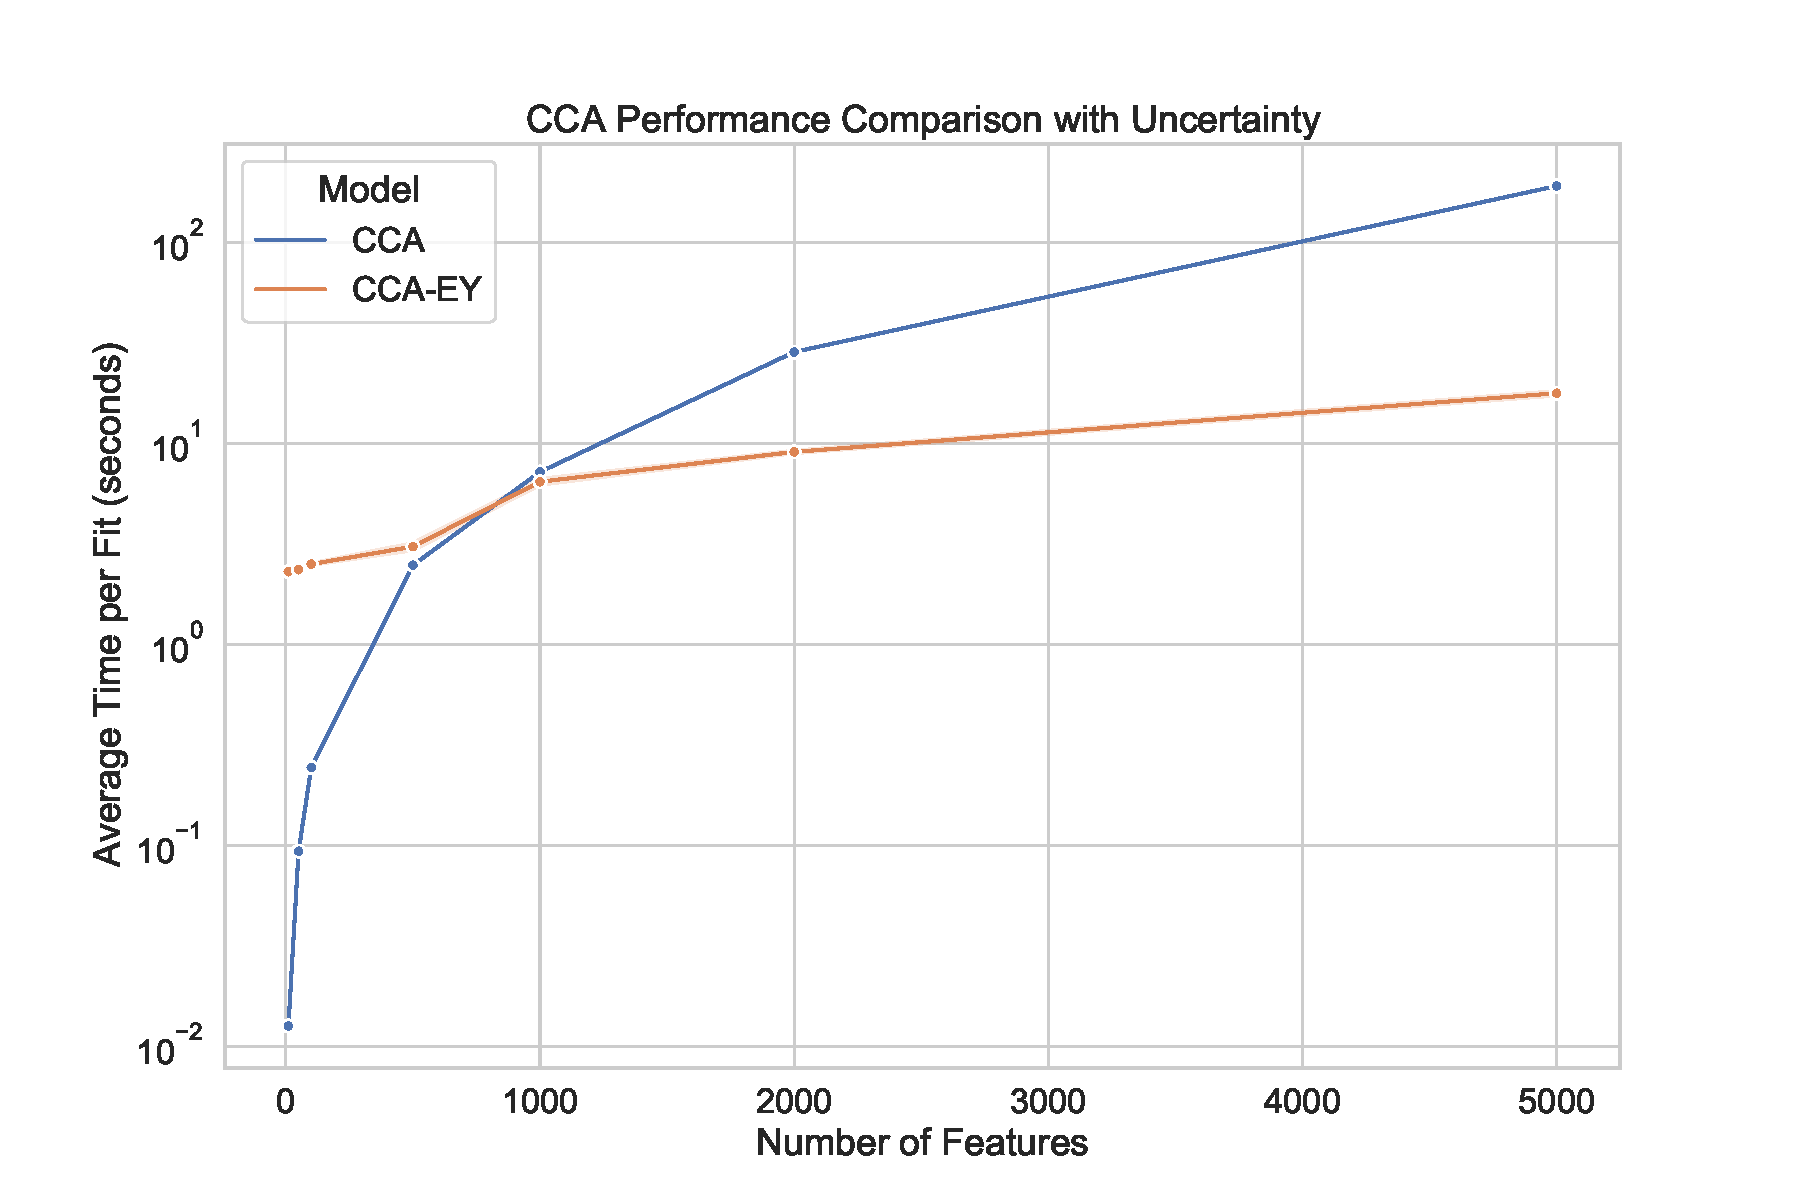
\includegraphics[width=0.8\textwidth]{figures/benchmarks/cca_comparison_log}
    \caption{Comparison of the time taken to solve CCA using \texttt{eigh} and our CCA-EY method.}
    \label{fig:cca-comparison}
\end{figure}

\subsection{Stochastic CCA on Real-World Datasets}
This experiment evaluates our CCA-EY method against two established baselines, $\gamma$-EigenGame \citep{gemp2022generalized} and SGHA \citep{chen2019constrained}, on real-world datasets. We aim to assess the algorithms' ability to handle high-dimensional data efficiently and accurately without prior dimensionality reduction.

\subsubsection{Datasets}
We employ two diverse datasets:

\begin{enumerate}
    \item \textbf{MediaMill} \citep{gemert2008visual}:
        \begin{itemize}
            \item \textbf{Content}: Paired features from videos and textual commentary
            \item \textbf{Objective}: Learn joint representations capturing visual-textual correlations
            \item \textbf{Size}: 25,800 test instances
            \item \textbf{Features}: 120 (video view) and 101 (commentary view)
        \end{itemize}
    
    \item \textbf{Split-CIFAR} \citep{meng2021online}:
        \begin{itemize}
            \item \textbf{Derivation}: CIFAR-10 images split in half
            \item \textbf{Objective}: Learn correlated representations of image halves
            \item \textbf{Size}: 50,000 training and 10,000 test instances
            \item \textbf{Features}: 32x16x3 for each view
        \end{itemize}
\end{enumerate}

\subsubsection{Experimental Setup}
\begin{itemize}
    \item \textbf{Training Duration}: Single epoch
    \item \textbf{Batch Sizes}: 5, 20, 50, 100
    \item \textbf{Hyperparameter Tuning}: Grid search using Weights and Biases \citep{wandb}
\end{itemize}

Table \ref{tab:hyperparameters} details the hyperparameter ranges explored for each method.

\begin{table}[h!]
    \centering
    \caption{Hyperparameter ranges for CCA methods}
    \label{tab:hyperparameters}
    \begin{tabular}{|l|l|}
        \hline
        Parameter             & Values              \\
        \hline
        Minibatch size        & 5, 20, 50, 100      \\
        Components            & 5                   \\
        Epochs                & 1                   \\
        Seeds                 & 1, 2, 3, 4, 5       \\
        Learning rate         & 0.01, 0.001, 0.0001 \\
        $\gamma$*             & 0.01, 0.1, 1, 10    \\
        \hline
    \end{tabular}
    \footnotesize{* $\gamma$ is only used for $\gamma$-EigenGame}
\end{table}

\subsubsection{Evaluation Metric}
We use the Proportion of Correlation Captured (PCC) metric:

\begin{equation}
\text{PCC} = \frac{\sum_{k=1}^K \rho_k}{\sum_{k=1}^K \rho_k^*},
\end{equation}

where:
\begin{itemize}
    \item $K$: Number of canonical components
    \item $\rho_k$: Correlations of estimated representations $Z\sps{i}=X^{(i)}\hat{U}^{(i)}$ on the test set
    \item $\rho_k^*$: Canonical correlations from full batch covariance matrices
\end{itemize}

In our notation:
\begin{itemize}
    \item $\rho_k = \MCCA_K(\hat{Z}\sps{1}, \hat{Z}\sps{2})$
    \item $\rho_k^* = \MCCA_K(X\sps{1}, X\sps{2})$
\end{itemize}

This metric efficiently tracks algorithm performance over time while minimizing computational overhead \citep{meng2021online, gemp2022generalized, ma2015finding, ge2016efficient}.

By comparing CCA-EY with $\gamma$-EigenGame and SGHA across these real-world datasets and various batch sizes, we aim to demonstrate the robustness and efficiency of our method in handling high-dimensional, complex data without the need for prior dimensionality reduction.

\subsubsection{Results and Observations}
Figure \ref{fig:corr_mediamill} compares the learning curves of the algorithms on the MediaMill dataset for various mini-batch sizes. CCA-EY consistently outperforms the baselines across all batch sizes. Figure \ref{fig:learningcurve_mediamill} provides a more detailed view of the learning curves for batch sizes 5 and 100, highlighting the superior performance of CCA-EY over time.
\begin{figure}
\centering
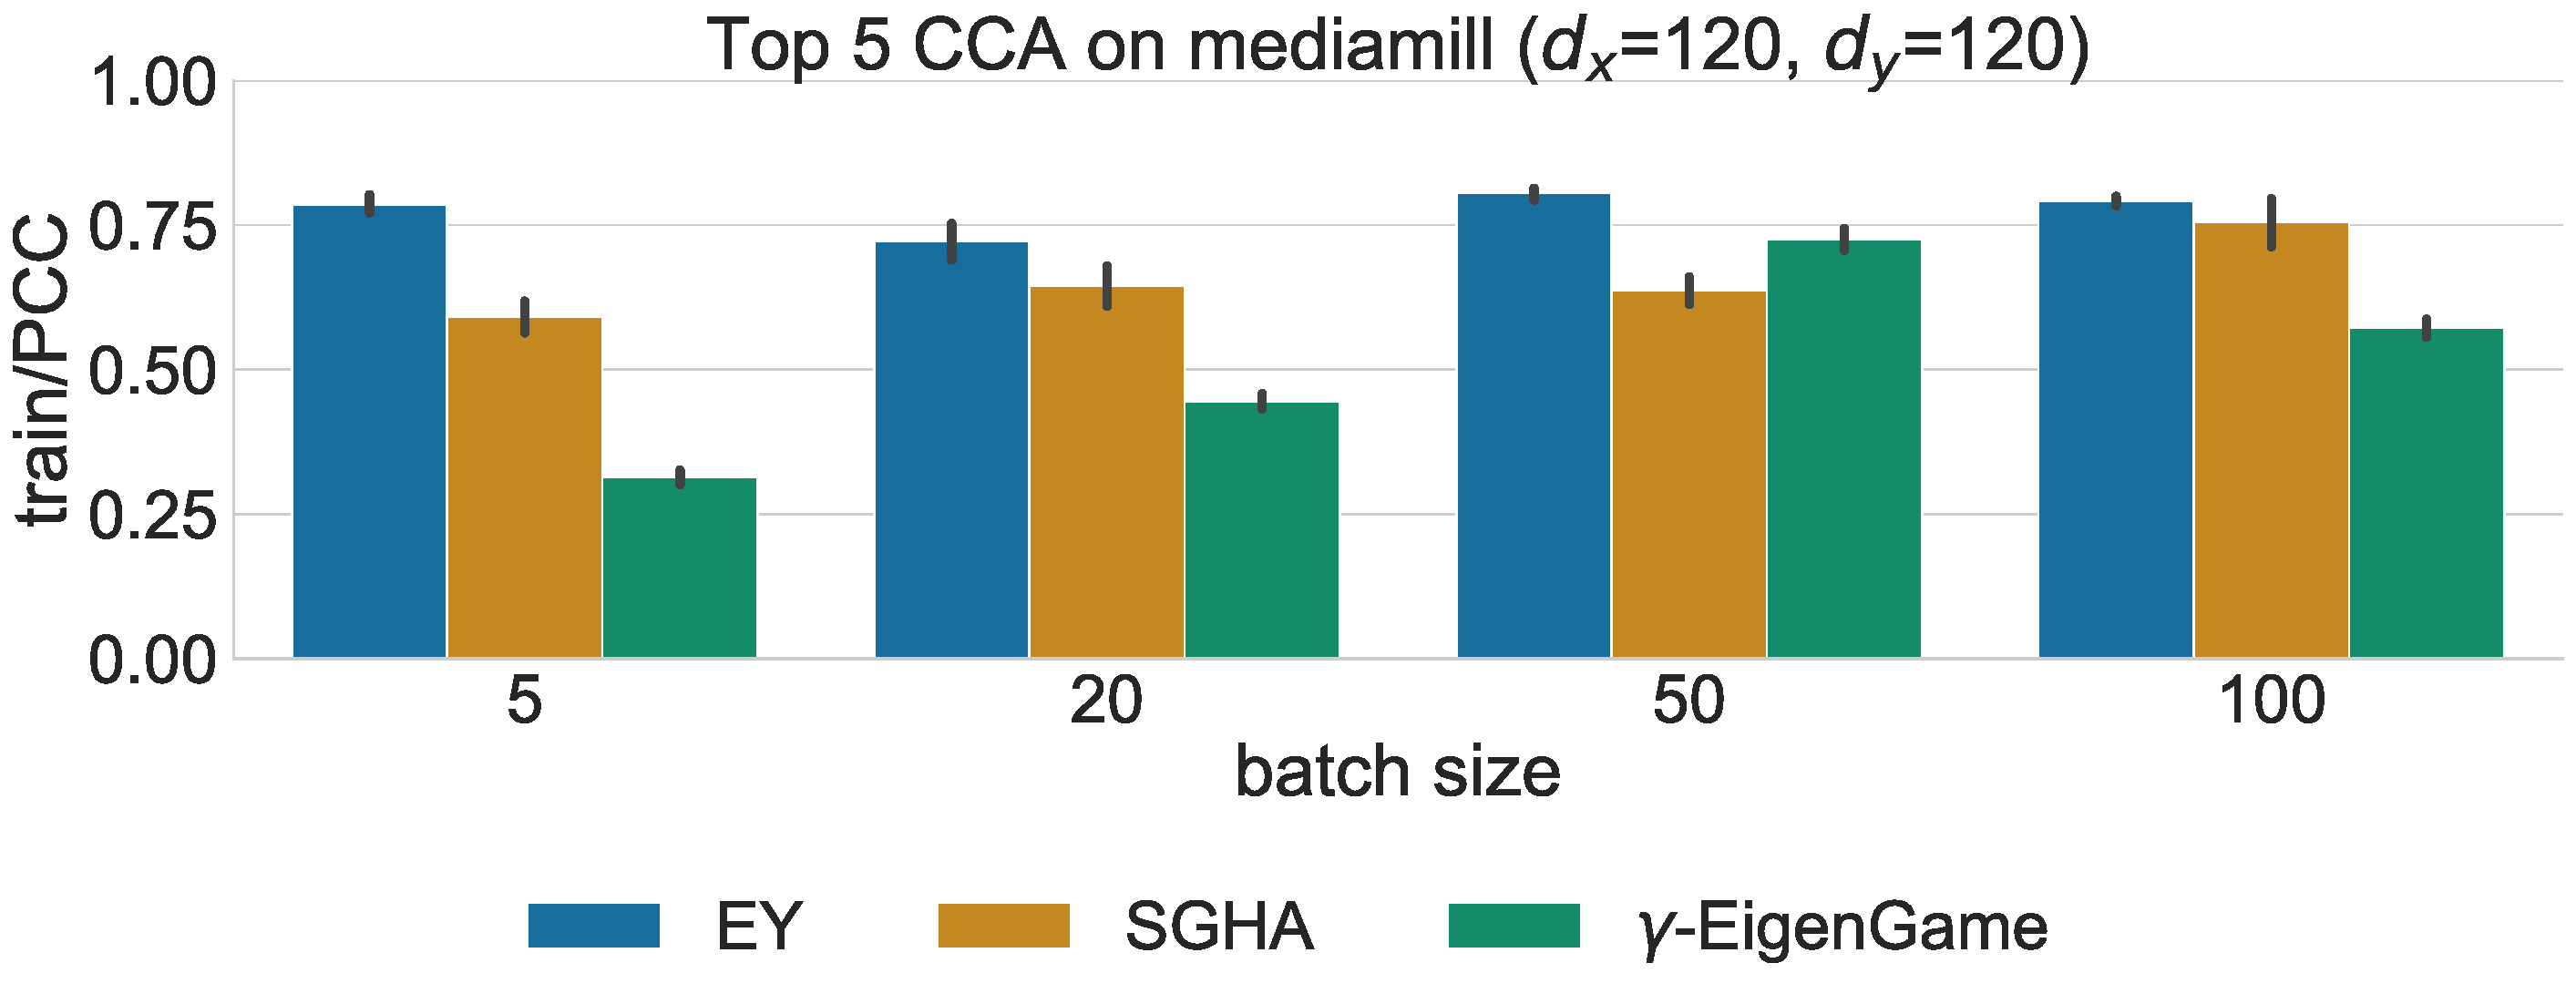
\includegraphics[width=0.8\textwidth]{figures/CCA/mediamill_models_different_batch_sizes}
\caption{Stochastic CCA on MediaMill using PCC: Performance across varying mini-batch sizes. Shaded regions represent $\pm$ one standard deviation around the mean of 5 runs.}
\label{fig:corr_mediamill}
\end{figure}
\begin{figure}
\centering
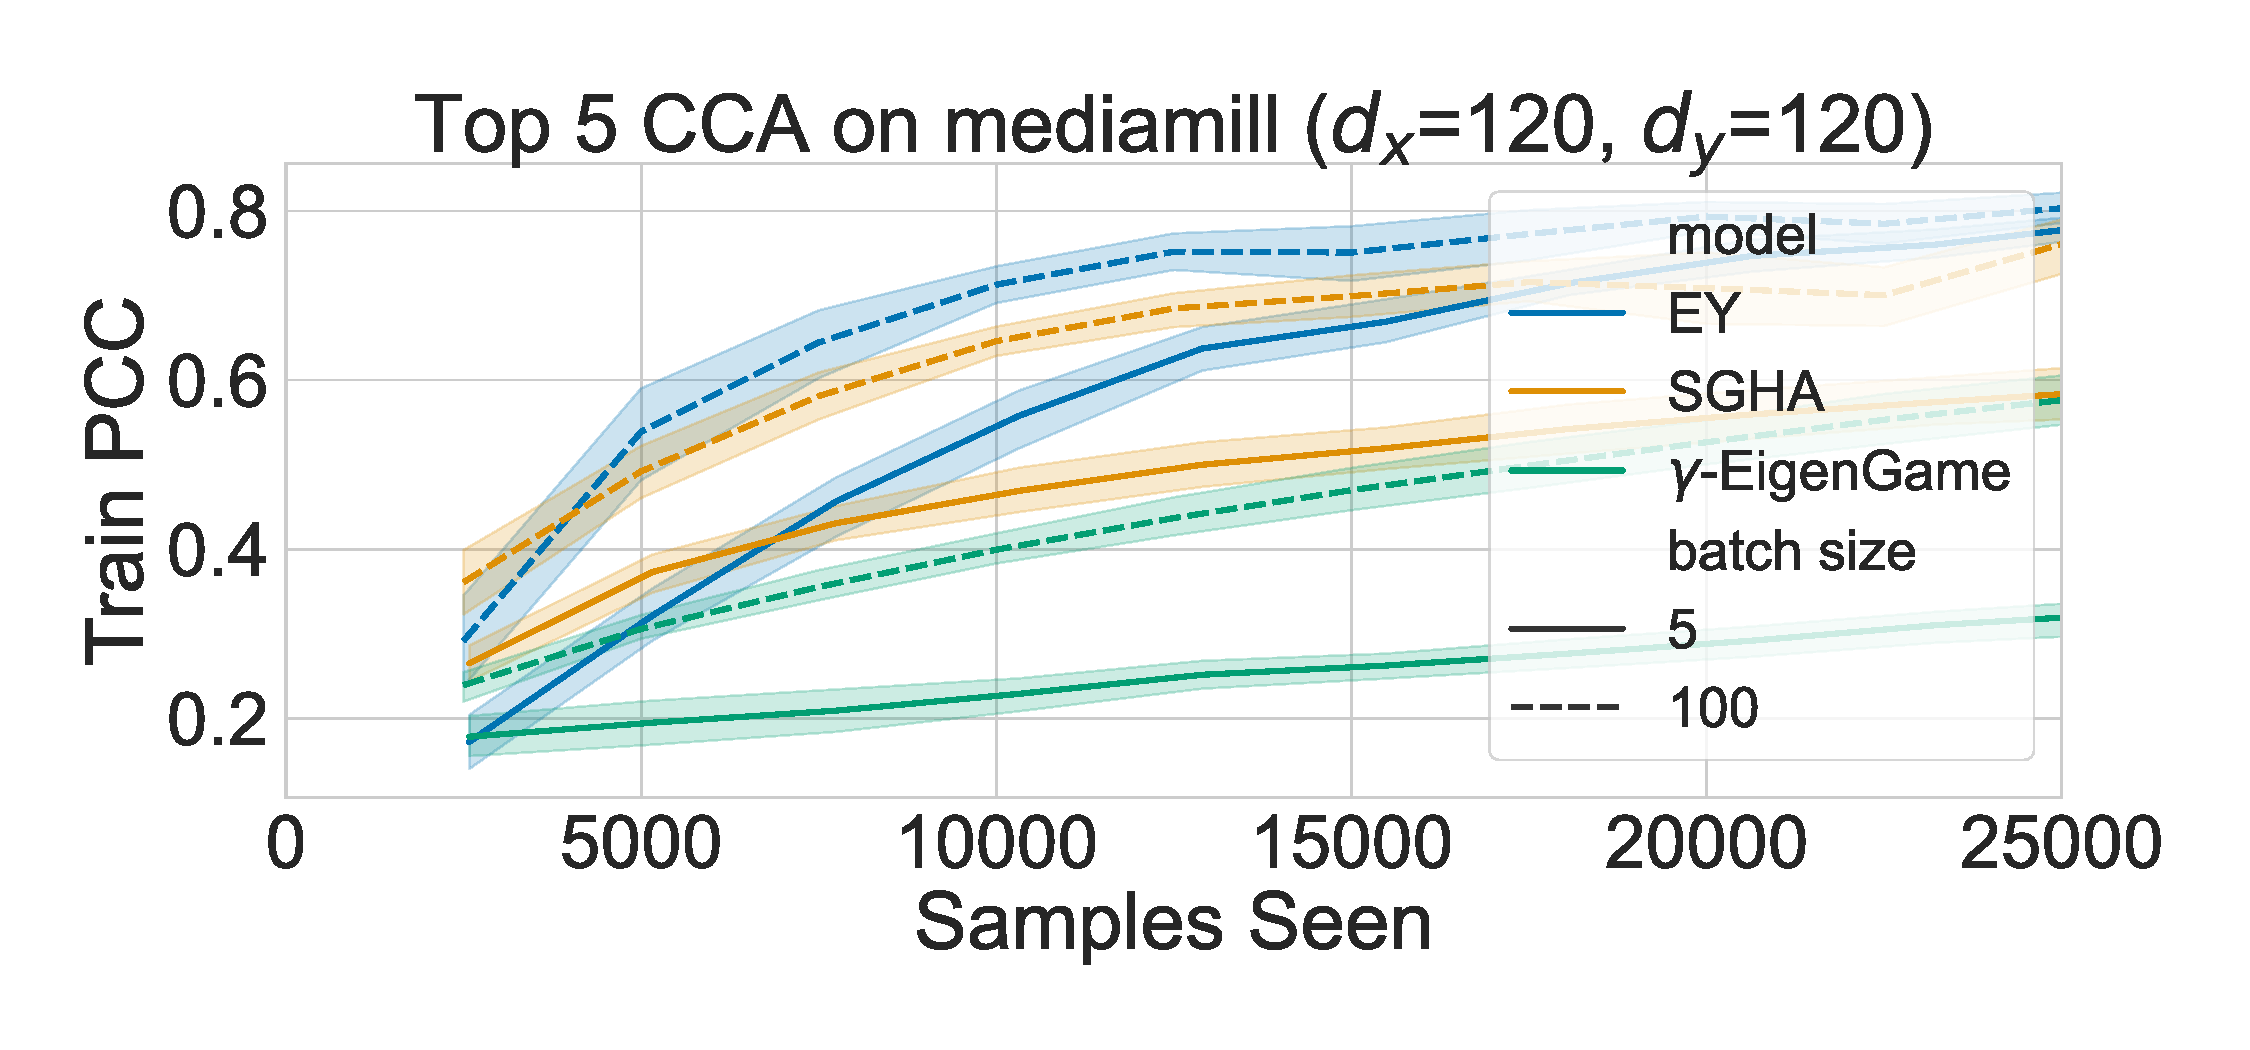
\includegraphics[width=0.8\textwidth]{figures/CCA/mediamill_allbatchsizes_pcc}
\caption{Stochastic CCA on MediaMill: Training progress over a single epoch for mini-batch sizes 5 and 100.}
\label{fig:learningcurve_mediamill}
\end{figure}
For the Split-CIFAR dataset, Figure \ref{fig:corr_cifar} shows the performance comparison across batch sizes, while Figure \ref{fig:learningcurve_cifar} presents the learning curves. The results reveal that $\gamma$-EigenGame underperforms compared to CCA-EY and SGHA, particularly for smaller batch sizes.
\begin{figure}
\centering
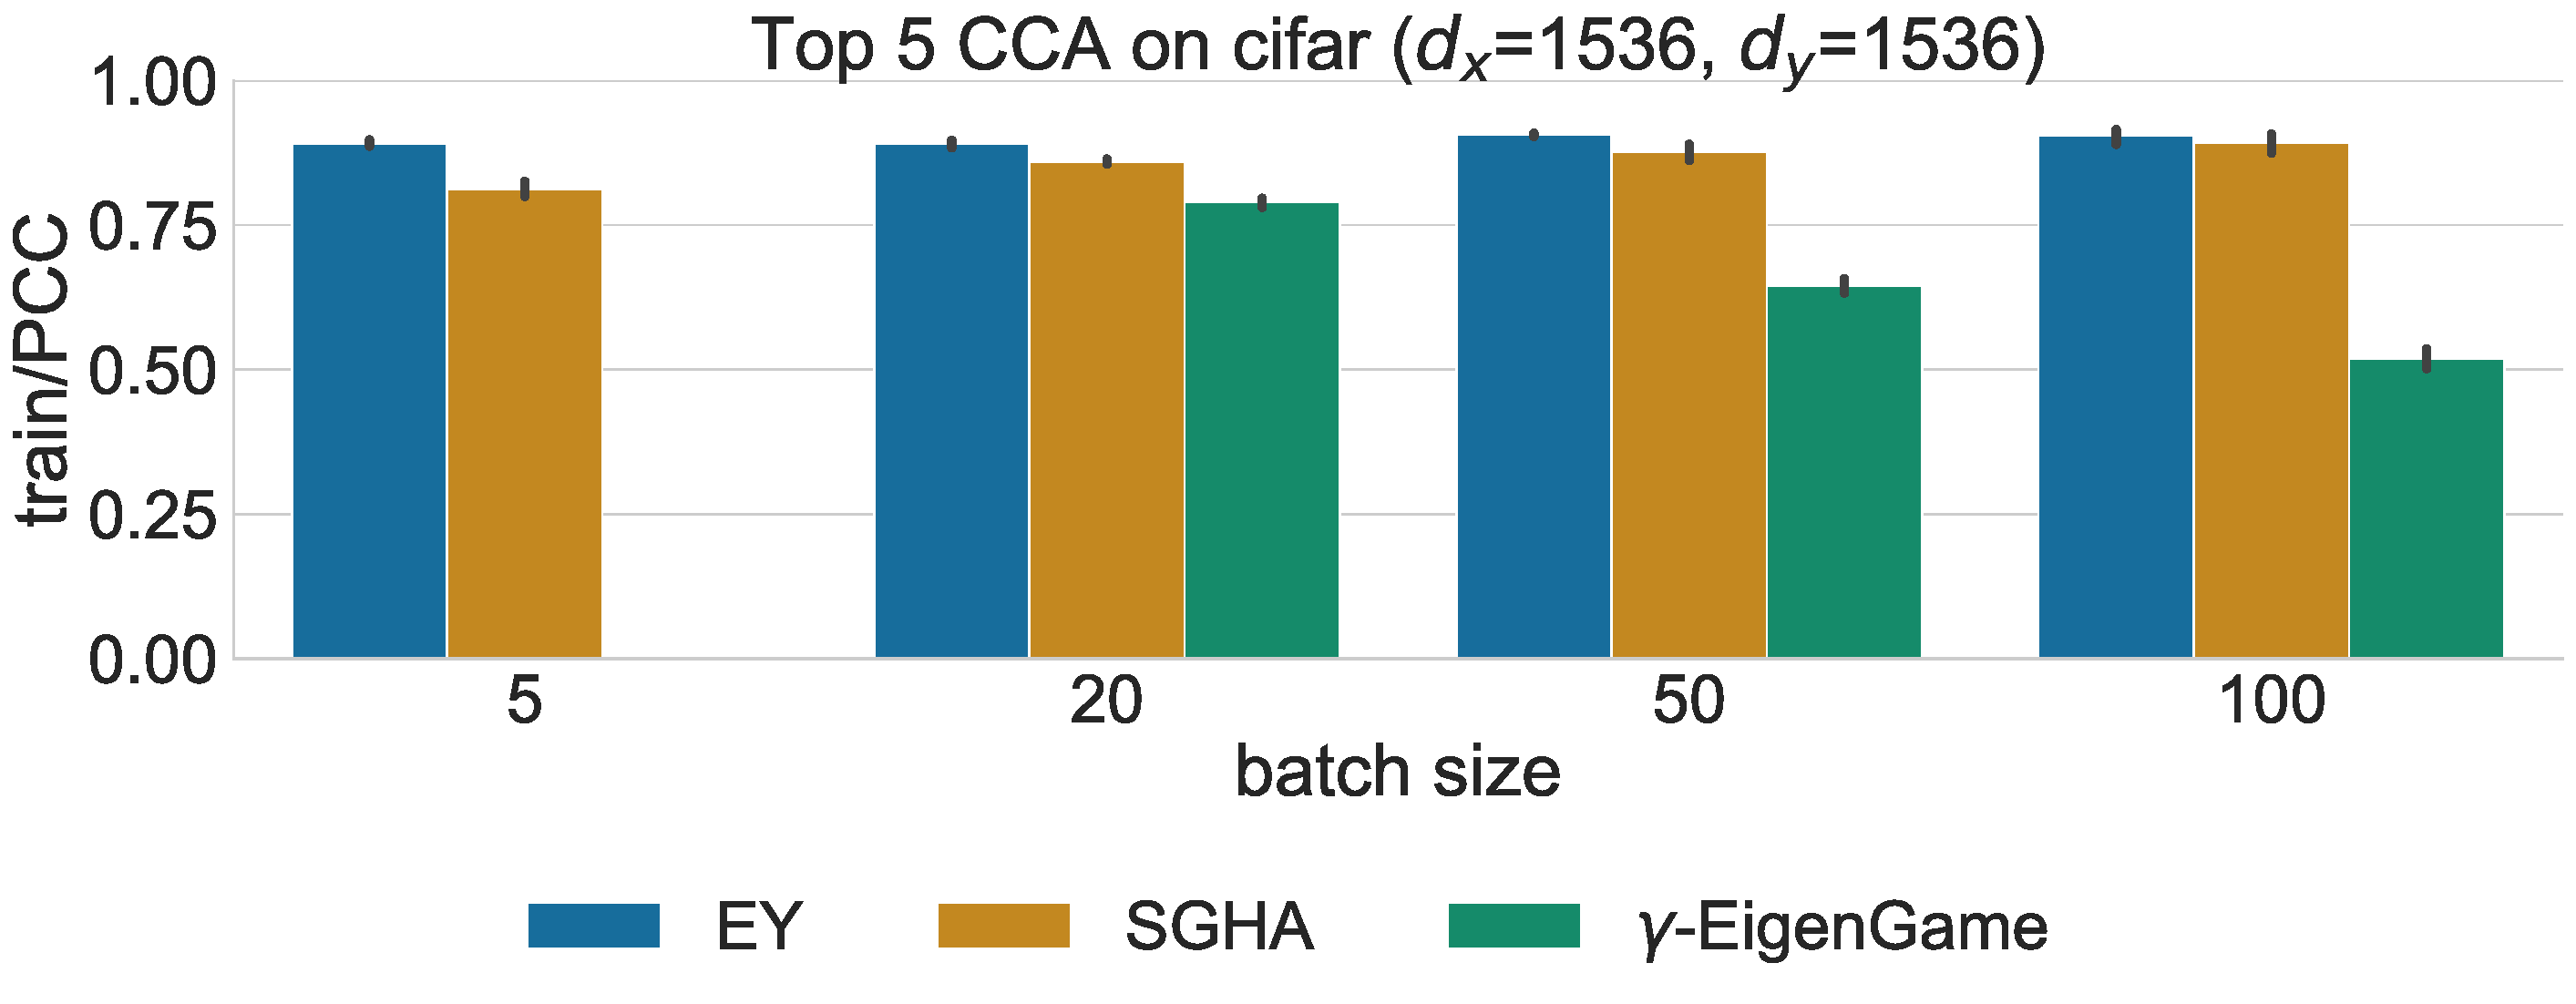
\includegraphics[width=0.8\textwidth]{figures/CCA/cifar_models_different_batch_sizes}
\caption{Stochastic CCA on Split-CIFAR using PCC: Performance across varying mini-batch sizes. Shaded regions represent $\pm$ one standard deviation around the mean of 5 runs.}
\label{fig:corr_cifar}
\end{figure}
\begin{figure}
\centering
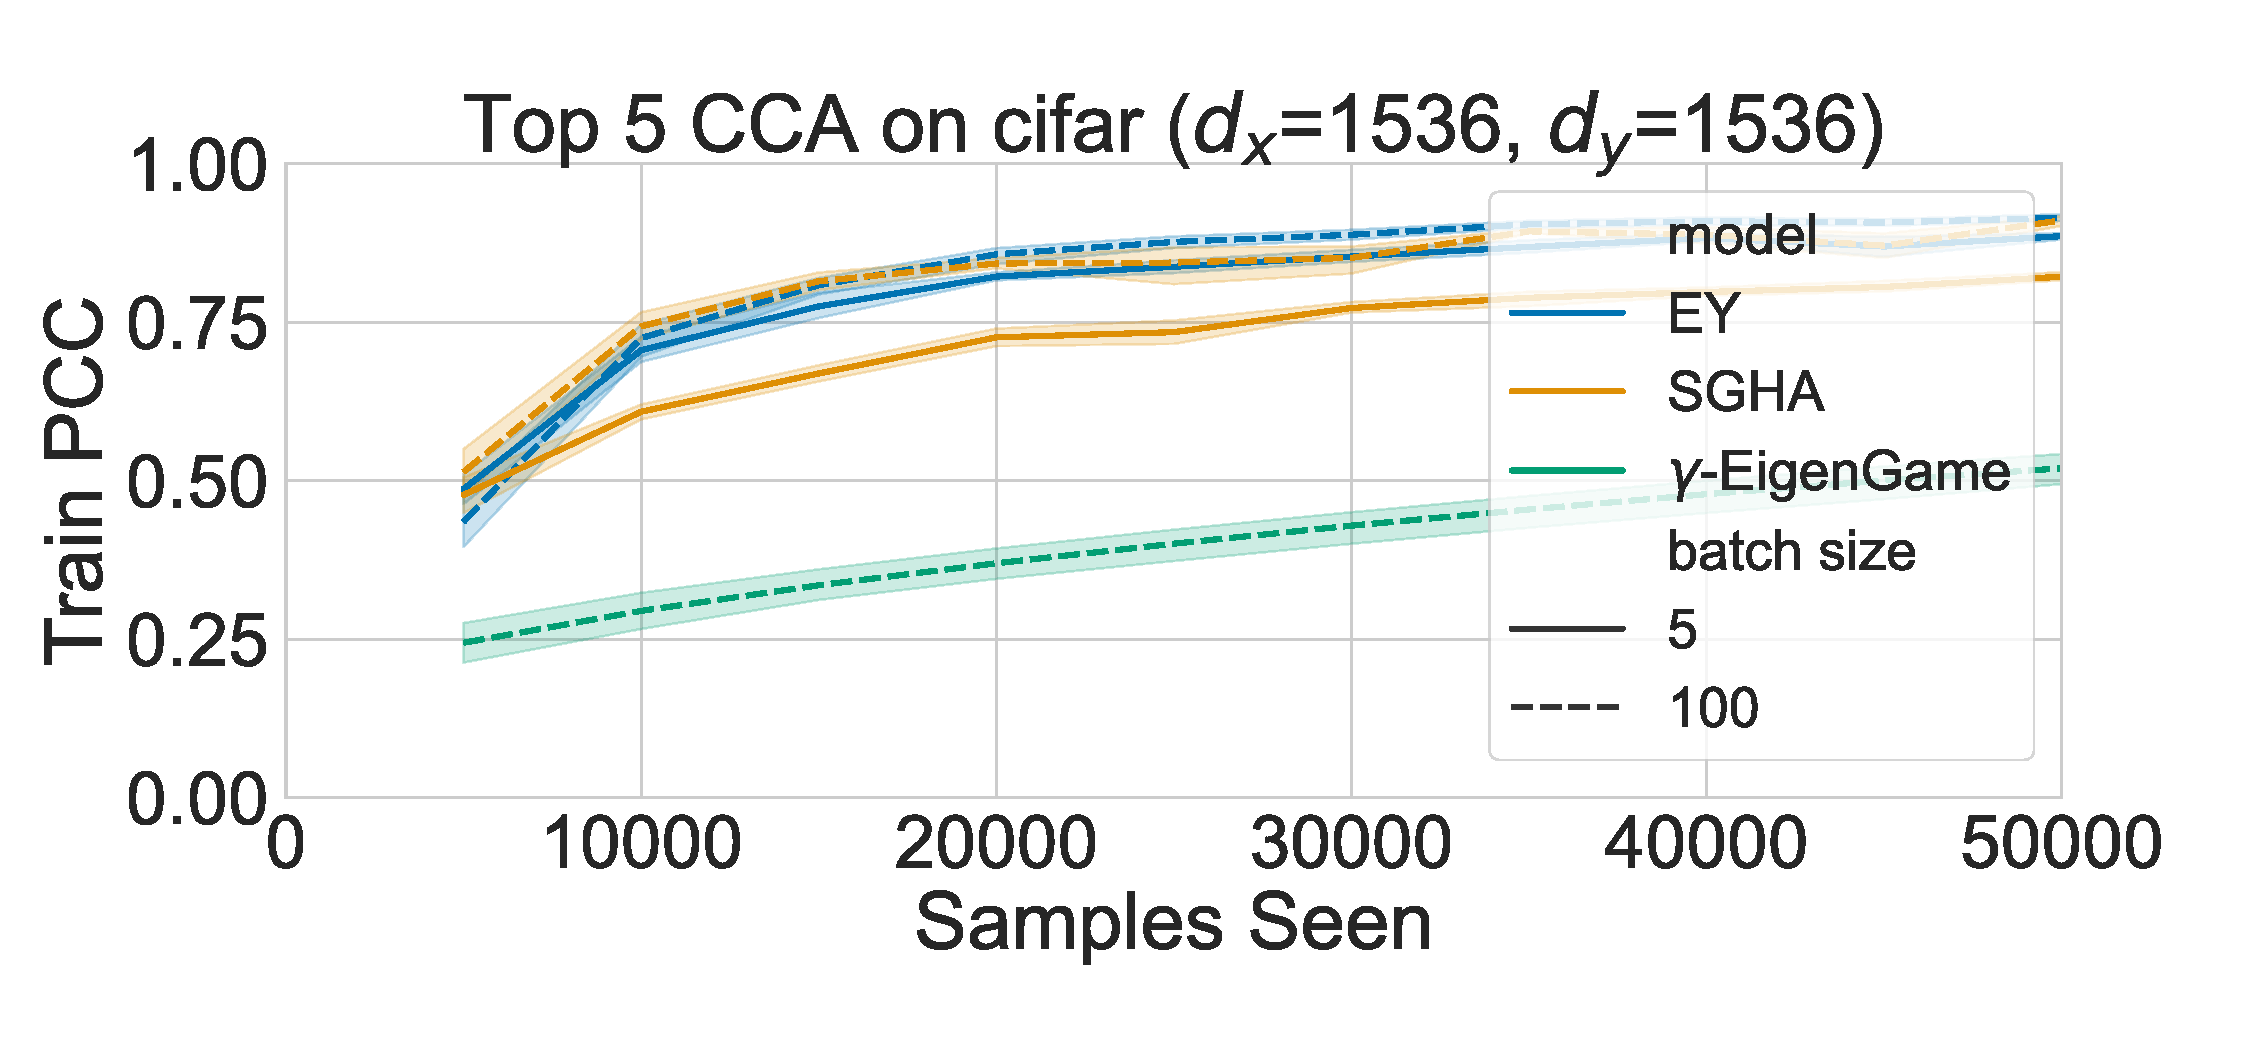
\includegraphics[width=0.8\textwidth]{figures/CCA/cifar_allbatchsizes_pcc}
\caption{Stochastic CCA on Split-CIFAR: Training progress over a single epoch for mini-batch sizes 5 and 100.}
\label{fig:learningcurve_cifar}
\end{figure}
These experiments demonstrate that our proposed CCA-EY method can achieve faster convergence with less hyperparameter tuning compared to the established baselines, making it a promising approach for practical applications involving high-dimensional data.

\subsection{Stochastic PLS on UK Biobank Data}
In this experiment, we showcase the scalability and efficiency of our Stochastic PLS method, PLS-EY, on an extremely high-dimensional imaging genetics dataset from the UK Biobank \citep{sudlow2015uk}.
\subsubsection{Data}
The UK Biobank is a large-scale biomedical database containing genetic and phenotypic data from over 500,000 participants. For this experiment, we use a subset of the data consisting of brain imaging features (82 regional volumes) and genetic variants (582,565 SNPs) for 33,333 subjects.
The brain imaging data was preprocessed using FreeSurfer \citep{Fischl2012} to extract gray-matter volumes for 66 cortical regions (based on the Desikan-Killiany atlas) and 16 subcortical regions. The effects of age, age squared, intracranial volume, sex, and the first 20 genetic principal components (to account for population structure) were regressed out from the brain features. Each brain region of interest (ROI) was then normalized by removing the mean and dividing by the standard deviation.
The genetic data was processed using PLINK \citep{Purcell2007}, retaining genetic variants with a minor allele frequency of at least 1% and a maximum missingness rate of 2%. Mean imputation was used to fill in missing values, and each variant was centered.
To generate measures of genetic disease risk, we calculated polygenic risk scores using PRSice \citep{PRSice2014}. Scores were computed with a p-value threshold of 0.05 using GWAS summary statistics for the following diseases: Alzheimer's \citep{Lambert2013}, Schizophrenia \citep{Trubetskoy2022}, Bipolar disorder \citep{Mullins2021}, ADHD \citep{Demontis2023}, ALS \citep{Van_Rheenen2021}, Parkinson's disease \citep{Nalls2019}, and Epilepsy \citep{International_League_Against_Epilepsy_Consortium_on_Complex_Epilepsies2018}.
\subsubsection{Experimental Setup}
We apply our PLS-EY method to the UK Biobank dataset, using a mini-batch size of 500 and training for 100 epochs with a learning rate of 0.0001. A key computational challenge in this experiment is maintaining orthogonality between the weight vectors $u_k$ in the PLS model, which is crucial for the method's effectiveness.
This approach allows us to handle the high-dimensional nature of the data while preserving the interpretability of the learned representations. To the best of our knowledge, this experiment represents the largest-scale PLS analysis of biomedical data to date, demonstrating the potential of our method to facilitate discoveries in extremely large datasets.
\subsubsection{Results and Observations}
Figure \ref{fig:UKBB_corr} shows the Pearson correlations among the PLS latent variables $Z_k$ derived from the UK Biobank data. We observe strong correlations between corresponding pairs of representations $Z^{(1)}_k$ and $Z^{(2)}_k$, and weak cross-correlations between $Z^{(1)}_k$ and $Z^{(2)}_i$ for $i \neq k$. This indicates that our PLS-EY model learns a coherent and orthogonal subspace.
\begin{figure}
\centering
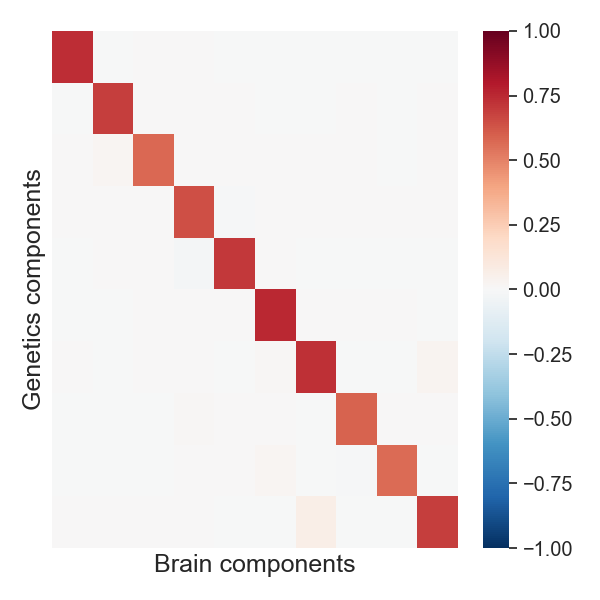
\includegraphics[width=0.6\textwidth,trim={0.8cm 0cm 0.3cm 0cm}]{figures/UKBB/cross_corr.png}
\caption{Pearson correlations among PLS latent variables $Z_k$ derived from UK Biobank data.}
\label{fig:UKBB_corr}
\end{figure}
Furthermore, we investigate the associations between the PLS brain representations $Z$ and the polygenic risk scores for various disorders, as shown in Figure \ref{fig:genetic_risk}. The results reveal significant correlations between the learned representations and genetic risk measures for several disorders, suggesting that the PLS subspace captures relevant information for genetic disease risk. This finding has important implications for biomedical research, as it demonstrates the ability of our method to uncover meaningful relationships in high-dimensional data.
\begin{figure}
\centering
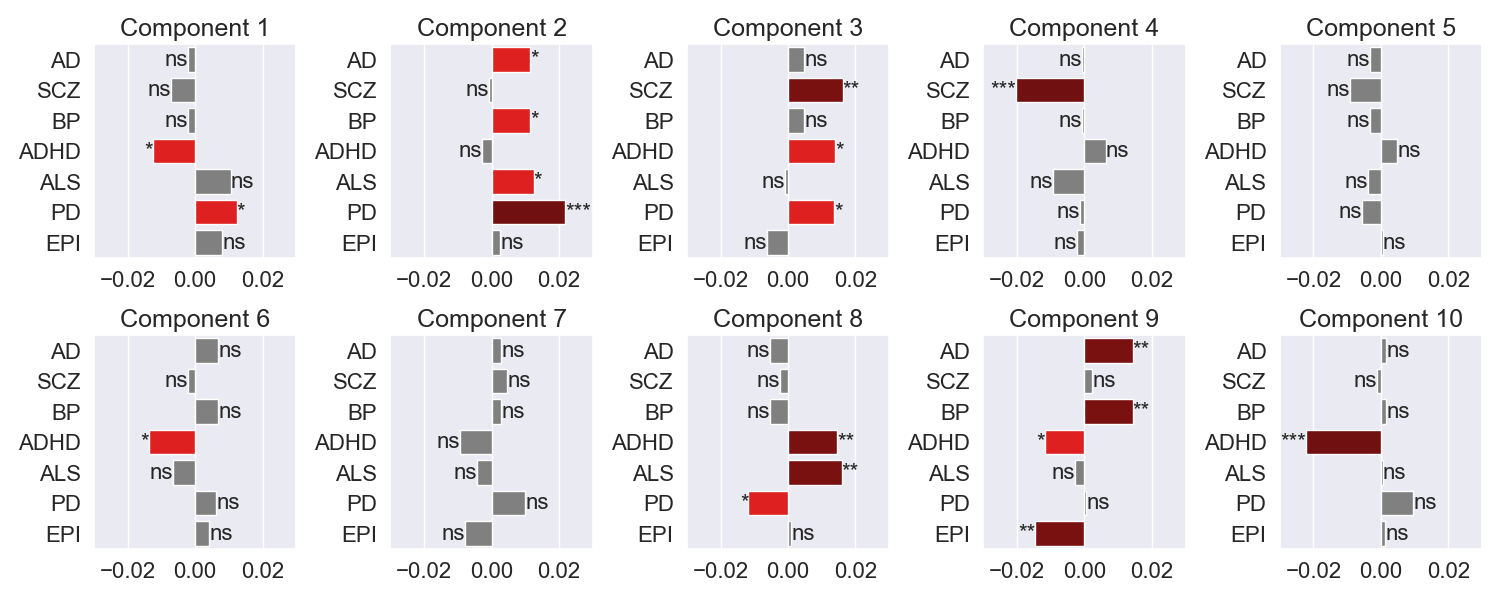
\includegraphics[width=0.99\textwidth,trim={0.5cm 0cm 0.7cm 0cm}]{figures/UKBB/prs_correlations.png}
\caption{Correlation between PLS brain representations $Z$ and genetic risk scores for various disorders. AD=Alzheimer's disease, SCZ=Schizophrenia, BP=Bipolar disorder, ADHD=Attention deficit hyperactivity disorder, ALS=Amyotrophic lateral sclerosis, PD=Parkinson's disease, EPI=Epilepsy. $\text{ns}: 0.05 < p \leq 1, \ast: 0.01 < p \leq 0.05, \ast\ast: 0.001 < p \leq 0.01, \ast\ast\ast: 0.0001 < p \leq 0.001$.}
\label{fig:genetic_risk}
\end{figure}
These results demonstrate the scalability of our PLS-EY method to extremely high-dimensional data and its ability to learn interpretable representations that capture biologically relevant information. The successful application of our method to the UK Biobank dataset highlights its potential to facilitate discoveries in large-scale biomedical studies.

\section{Discussion and Limitations}\label{sec:discussion}

\subsection{Limitations}

This chapter presents a comprehensive exploration and development of novel algorithms for Canonical Correlation Analysis (CCA) and Partial Least Squares (PLS), focusing on scalability and efficiency in high-dimensional and large-scale datasets.
Our approach introduces the Eckhart-Young (EY) inspired objectives for Generalized Eigenvalue Problems (GEPs) and their application in stochastic or data-streaming settings, paving the way for more efficient and scalable solutions to classical subspace learning problems.

Our proposed CCA-EY and PLS-EY methods demonstrate significant advancements over traditional approaches in handling the computational complexity and scalability issues inherent in high-dimensional data.
By reformulating the CCA and PLS objectives, we provide a path to efficiently analyze large datasets, which was previously infeasible due to computational limitations.
The empirical evaluation on diverse datasets, including MediaMill, Split-CIFAR-10, and the UK Biobank, not only validates the effectiveness of our methods but also highlights their superiority in convergence speed and robustness to hyperparameter tuning.

The results from the MediaMill and Split-CIFAR-10 datasets underscore the potential of CCA-EY in achieving faster convergence with minimal hyperparameter tuning, a crucial factor for practical applications.
This advantage is particularly pronounced when comparing our method to established baselines like $\gamma$-EigenGame and SGHA. Additionally, the application of our methods to the UK Biobank dataset represents a breakthrough in the analysis of imaging genetics data, showcasing the capability of PLS-EY to manage extraordinarily high-dimensional data while extracting meaningful and interpretable representations.

Furthermore, our methods' ability to capture relevant information for genetic disease risk, as evidenced in the UK Biobank study, opens new avenues for biomedical research.
The significant associations between the PLS representations and genetic risk measures for various disorders provide valuable insights into the genetic mechanisms underlying diseases and brain morphometry.

\section{Future Work: Proximal Gradient Descent for Regularized GEPs}

While our current work focuses on unregularized GEPs, future research will extend our approach to incorporate complex regularization terms efficiently. We propose using proximal gradient descent, a method well-suited for optimizing loss functions comprising a smooth, differentiable component and a non-smooth regularization term.

\subsection{Regularized Objective for GEP-EY}

We aim to extend the GEP-EY framework by integrating specific regularization terms directly into the loss function. The revised loss function, denoted as $\mathcal{L}_{\text{Reg-GEP-EY}}(\theta)$, will incorporate regularization terms $R_i(\theta^{(i)})$ for each view $i$:

\begin{align}
    \mathcal{L}_{\text{Reg-GEP-EY}}(\theta) = \mathcal{L}_{\text{EY}}(\theta) + \sum_{i=1}^I \lambda_i R_i(\theta^{(i)}),
\end{align}

where $\mathcal{L}_{\text{EY}}(\theta)$ is our original GEP-EY loss function, $\lambda_i$ are regularization parameters, and $R_i(\theta^{(i)})$ are view-specific regularization terms. This formulation allows for the inclusion of non-smooth penalties such as L1-norm or Total Variation (TV), which can enforce sparsity or structural constraints on the learned representations.

\subsection{Proximal Gradient Descent Algorithm}

The proximal gradient descent algorithm for optimizing the regularized GEP-EY objective alternates between a gradient step on the smooth part of the loss and a proximal step for the non-smooth regularization terms:

\begin{align}
\theta^{(i)}_{t+1} &= \text{prox}_{\alpha \lambda_i R_i}\left(\theta^{(i)}_t - \alpha \nabla_{\theta^{(i)}} \mathcal{L}_{\text{EY}}(\theta_t)\right),
\end{align}

where $\text{prox}_{\alpha \lambda_i R_i}(\cdot)$ denotes the proximal operator for the regularization term $R_i$ with parameter $\lambda_i$, and $\alpha$ is the learning rate. The proximal operator is defined as:

\begin{align}
\text{prox}_{\alpha \lambda_i R_i}(v) = \arg \min_u \left( R_i(u) + \frac{1}{2\alpha} \|u - v\|_2^2 \right).
\end{align}

This approach effectively balances the influence of the smooth loss function gradient and the geometry imposed by the regularization, making it robust to the inclusion of complex constraints in GEP optimization.

\subsection{Potential Applications and Benefits}

The incorporation of proximal gradient descent into our GEP-EY framework opens up several exciting possibilities:

\begin{enumerate}
    \item \textbf{Sparse CCA:} By using L1 regularization, we can encourage sparsity in the learned representations, leading to more interpretable results.
    \item \textbf{Structured CCA:} Total Variation regularization can enforce spatial or temporal smoothness in the representations, which is particularly useful for neuroimaging or time-series data.
    \item \textbf{Multi-view learning with heterogeneous regularization:} Different regularization terms can be applied to different views, allowing for more flexible modeling of complex multi-view data.
    \item \textbf{Improved generalization:} Appropriate regularization can help prevent overfitting, especially in high-dimensional, low-sample size scenarios.
\end{enumerate}

Future work will focus on implementing this proximal gradient descent approach, developing efficient algorithms for specific regularization terms, and evaluating its performance on various real-world datasets.

% \subsection{Regularized Objective for GEP-EY}

% Our future initiatives will enhance CCA, PCA and PLS by incorporating proximal gradient descent for efficient handling of complex regularization terms. This methodology is ideally suited for scenarios where the loss function comprises a smooth, differentiable component plus a non-smooth regularization term. The proximal gradient technique uses a gradient step followed by a proximal step, enabling effective management of non-smooth penalties such as L1-norm or Total Variation (TV), which are instrumental in enforcing sparsity and structural constraints.

% \subsubsection{Objective Formulation with Regularization}

% We aim to modify the CCA framework by integrating specific regularization terms directly into the loss function of the Generalized Eigenvalue Problem (GEP). The revised loss function, denoted as $\mathcal{L}_{\text{Proximal CCA-EY}}(\mathbf{U}_1, \mathbf{U}_2)$, will incorporate the regularization terms $R_1(\mathbf{U}_1)$ and $R_2(\mathbf{U}_2)$, enabling the optimization of CCA with additional constraints. The objective function for Proximal CCA-EY will be defined as:

% \begin{align*}
%     \mathcal{L}_{\text{Proximal CCA-EY}}(\mathbf{U}_1, \mathbf{U}_2) &= \mathcal{L}_{\text{EY}}(\mathbf{U}_1, \mathbf{U}_2)
%     + \lambda_1 R_1(\mathbf{U}_1) + \lambda_2 R_2(\mathbf{U}_2),
% \end{align*}

% where $\mathcal{L}^{\text{Proximal CCA-EY}}$ represents the Proximal CCA-EY loss function, $\lambda_1$ and $\lambda_2$ are regularization parameters, and $R_1(\mathbf{U}_1)$ and $R_2(\mathbf{U}_2)$ are the regularization terms for each view.

% \subsubsection{Proximal Gradient Descent Mechanism}

% The proximal gradient updates for this augmented CCA formulation are specified as:

% \begin{align}
% \mathbf{U}1^{(t+1)} &= \text{prox}{\alpha \lambda_1 R_1}(\mathbf{U}_1^{(t)} - \alpha \nabla{\mathbf{U}_1} \mathcal{L}^{\text{EY}}(\mathbf{U}_1^{(t)}, \mathbf{U}_2^{(t)})), \
% \mathbf{U}2^{(t+1)} &= \text{prox}{\alpha \lambda_2 R_2}(\mathbf{U}_2^{(t)} - \alpha \nabla{\mathbf{U}_2} \mathcal{L}^{\text{EY}}(\mathbf{U}_1^{(t)}, \mathbf{U}_2^{(t)})),
% \end{align}

% where $\text{prox}_{\alpha \lambda_i R_i}(\mathbf{v})$ denotes the proximal operator for the regularization term $R_i$ with parameter $\lambda_i$, and $\alpha$ represents the learning rate. Note that the gradients $\nabla{\mathbf{U}_1} \mathcal{L}^{\text{EY}}(\mathbf{U}_1^{(t)}, \mathbf{U}_2^{(t)})$ and $\nabla{\mathbf{U}_2} \mathcal{L}^{\text{EY}}(\mathbf{U}_1^{(t)}, \mathbf{U}_2^{(t)})$ are computed only for the smooth part of the loss function, i.e., $\mathcal{L}^{\text{EY}}(\mathbf{U}_1, \mathbf{U}_2)$, and do not include the regularization terms.

% The proximal operator is defined as solving:

% \begin{align*}
% \text{prox}{\alpha \lambda_i R_i}(\mathbf{v}) = \arg \min\mathbf{u} \left( R_i(\mathbf{u}) + \frac{1}{2\alpha} |\mathbf{u} - \mathbf{v}|_2^2 \right).
% \end{align*}

% This update effectively balances the influence of the gradient of the smooth loss function and the geometry imposed by the regularization, making the approach robust to the inclusion of complex constraints in the optimization of CCA.

% \subsubsection{Efficiency and Applicability}

% The proximal gradient descent method excels in large-scale optimization challenges where traditional techniques struggle due to the presence of non-smooth terms. By separating the optimization of the smooth component from the non-smooth regularization, proximal steps can be efficiently computed, particularly when $R_i$ allows a straightforward proximal formulation.

\subsection{Conclusion}

In summary, this chapter contributes to the fields of machine learning and multiview data analysis by introducing scalable and efficient solutions for CCA and PLS, applicable in a variety of domains, including but not limited to neuroimaging and genetics.
Our work not only addresses significant computational challenges but also lays the groundwork for future research and practical applications in analyzing large-scale, high-dimensional datasets.